% !TEX encoding = UTF-8
%Koma article
\documentclass[fontsize=12pt,paper=letter,twoside]{scrartcl}
\usepackage{float}
\usepackage{listings}

%Standard Pre-amble
\usepackage[top=4cm,bottom=4cm,left=3cm,right=3cm,asymmetric]{geometry}
%\geometry{landscape}                % Activate for for rotated page geometry
%\usepackage[parfill]{parskip}    % Begin paragraphs with an empty line rather than an indent
\usepackage[table,xcdraw]{xcolor}
\usepackage{graphicx}

\usepackage{amsmath}
\usepackage{amssymb}
\usepackage{epstopdf}
\DeclareGraphicsRule{.tif}{png}{.png}{`convert #1 `dirname #1`/`basename #1 .tif`.png}
% Listings needs package courier
\usepackage{listings} % Needs 
\usepackage{courier}

\usepackage[framemethod=TikZ]{mdframed}
\usepackage{url}

\usepackage{sty/bsymb} %% Event-B symbols
\usepackage{sty/eventB} %% REQ and ENV
\usepackage{sty/calculation}

%Maths
\usepackage{amssymb,amsmath}
\def\Fl{\mathbb{F}}
\def\Rl{\mathbb{R}}
\def\Nl{\mathbb{N}}
\def\Bl{\mathbb{B}}
\def\St{\mathbb{S}}
\newcommand{\ovr}{\upharpoonright}
\newcommand{\var}[1]{\textit{#1}}
%Useful definitions
\newcommand{\mv}[1]{\textit{m\_#1}}
\newcommand{\cv}[1]{\textit{c\_#1}}
\newcommand{\degree}[1]{^{\circ}\mathrm{#1}}
%\newcommand{\comment}[1]{{\footnotesize \quad\texttt{--}\textrm{#1}}}
\newcommand{\im}[1]{i\texttt{-\!#1}}

\usepackage[headsepline]{scrpage2}
\pagestyle{scrheadings}
\ihead[]{\small EECS4312 Report1}
\ohead[]{\small \thepage}
\cfoot[]{}
\ofoot[]{}


%%%%PVS environment%%%%%%%%%%%%%%%%%%%
\lstnewenvironment{pvs}[1][]
    {\lstset{#1,captionpos=b,language=pvs,
    mathescape=true,
    basicstyle=\small\ttfamily,
    numbers=none,
    frame=single,
    % numberstyle=\tiny\color{gray},
    % backgroundcolor=\color{lightgray},
    firstnumber=auto
    }}
    {}
 %%%%%%%%%%%%%%%%%%%%%%%%%%%%%%%%
 
%%%%Verbatim environment%%%%%%%%%%%%%%%%%%%
\lstnewenvironment{code}[1][]
    {\lstset{#1,captionpos=b,
    mathescape=true,
    basicstyle=\small\ttfamily,
    numbers=none,
    frame=single,
    % numberstyle=\tiny\color{gray},
    % backgroundcolor=\color{lightgray},
    firstnumber=auto
    }}
    {}

% \newenvironment{boxed}[1]
%    {\begin{center}
%    #1\\[1ex]
%    \begin{tabular}{|p{0.9\textwidth}|}
%    \hline\\
%    }
%    { 
%    \\\\\hline
%    \end{tabular} 
%    \end{center}
%    }
 %%%%%%%%%%%%%%%%%%%%%%%%%%%%%%%%
 
 %Text in a box
\newenvironment{textbox}
    {\begin{center}
    \begin{tabular}{|p{0.9\textwidth}|}
    \hline\\
    }
    { 
    \\\\\hline
    \end{tabular} 
    \end{center}
    }

\usepackage{hyperref}

%Highlight \hl{}
\usepackage{soul}

\usepackage{enumitem}
\newlist{mylist}{itemize}{1}
\setlist[mylist]{label=\textbullet,leftmargin=1cm,nosep}

\usepackage{multirow}

% Reduce space between figure and caption
%\usepackage{caption}
%\captionsetup[table]{font=small,skip=0pt}     %% Adjust here
%or equivalently 
\usepackage[font=small,skip=4pt]{caption}
%Useful definitions
%\newcommand{\mv}[1]{\textit{m\_#1}}
%\newcommand{\cv}[1]{\textit{c\_#1}}
%\newcommand{\degree}[1]{^{\circ}\mathrm{#1}}
%\newcommand{\comment}[1]{{\footnotesize \quad\texttt{--}\textrm{#1}}}

% Set the header
\ihead[]{\small EECS4090 Project}


%%%%%%%%%%%%Enter your names here%%%%%%%%
\author{\textbf{Edward Vaisman}
\and \textbf{Sadman Sakib Hasan}
}
%%%%%%%%%%%%%%%%%%%%%%%%%%%%%%%%

\date{\today} % Display a given date or no date

\begin{document}
\title{Grad Apps 2.0 Requirements Documentation}
\maketitle

\newpage

\section*{Revisions}

%%%%%%%%%%%%Table of revisions%%%%%%%%
\begin{tabular}{|l|l|p{3in}|}
\hline
Date & Revision & Description \\ 
\hline
9 October, 2017
& 1.0
& \begin{mylist}
\item Fix grammars
\item Look into each research group for field of interest(s)
\end{mylist} \\
\hline
17 October, 2017
& 1.1
& Fix additional grammars \\
\hline
23 October, 2017
& 2.0
& \begin{mylist}
\item Apply new list of field of interest(s) conducted from the questionnaire
\item Further elicitation from the GPA and GPD
\end{mylist} \\ 
\hline
30 November, 2017
& 3.0
& Add complete use case diagrams, textual description for all specs \\ 
\hline
5 December, 2017
& 4.0
& \begin{mylist}
\item Add use case diagrams for each roles
\item Include additional R descriptions for optional deliverables
\item Include additional Use Case Textual Descriptions
\end{mylist} \\  
\hline
9 December, 2017
& 5.0
& Add abstract UI grammar and acceptance tests \\
\hline
29 December, 2017
& 6.0
& \begin{mylist}
\item Add system invariants
\item Reorganize E/R descriptions (seperated into usecases)
\item Fix UI grammar and acceptance tests
\end{mylist} \\  
\hline
2 January,  2017
& 7.0
& \begin{mylist}
\item Updated Use Case Textual Descriptions 
\item Re-organized E/R descriptions
\item Added error list and success list messages
\item General typo fixes
\item Added more system goals
\end{mylist} \\  
\hline
\end{tabular}
%%%%%%%%%%%%%%%%%%%%%%%%%%%%%%%%

\newpage

%%%%%%%%%%%%%%%%%%%%%%%%%%%%%%%
\tableofcontents
\listoffigures
\listoftables
\newpage


%%%%Rest of your document goes here%%%%%%%%%%%%%%%%%%%

\clearpage
\section{System Overview}

Having a post graduate degree on one's resume is always appealing to their future employer, let it be working in the industry or continuing studies to achieve a doctoral status. When applying for a postgraduate program, applicants spend a lot of their time gathering different levels of information (transcripts, letter of recommendation, resume and etc.) required for admission. Once an application has been submitted, the graduate program analyses the information to find the best candidate for each program.

Analysing that level of dense information can be challenging at times and to avoid loss of any information, it is best practice to automate this process as much as possible. In order to achieve that goal, a \emph{concise} and \emph{simple} Business System is required that can ease out the manual work.

The situation of the graduate program in Electrical Engineering and Computer Science (EECS) is very similar. The current system our client has involves a lot of manual work. The centre of this process is the Graduate Program Director (GPD) and Graduate Program Assistant (GPA) who plays a major role in all applications regardless of the applicant being admitted or rejected.

Our client requires a more robust and concise system that will enable them to \emph{automate} the selection of the best candidate into the program \emph{minimizing} the manual work to be done. The following diagram outlines the institutions faculty member hierarchy. Our client are the members of \textbf{The EECS Graduate Program}.

\begin{figure}[!htb]
\begin{center}
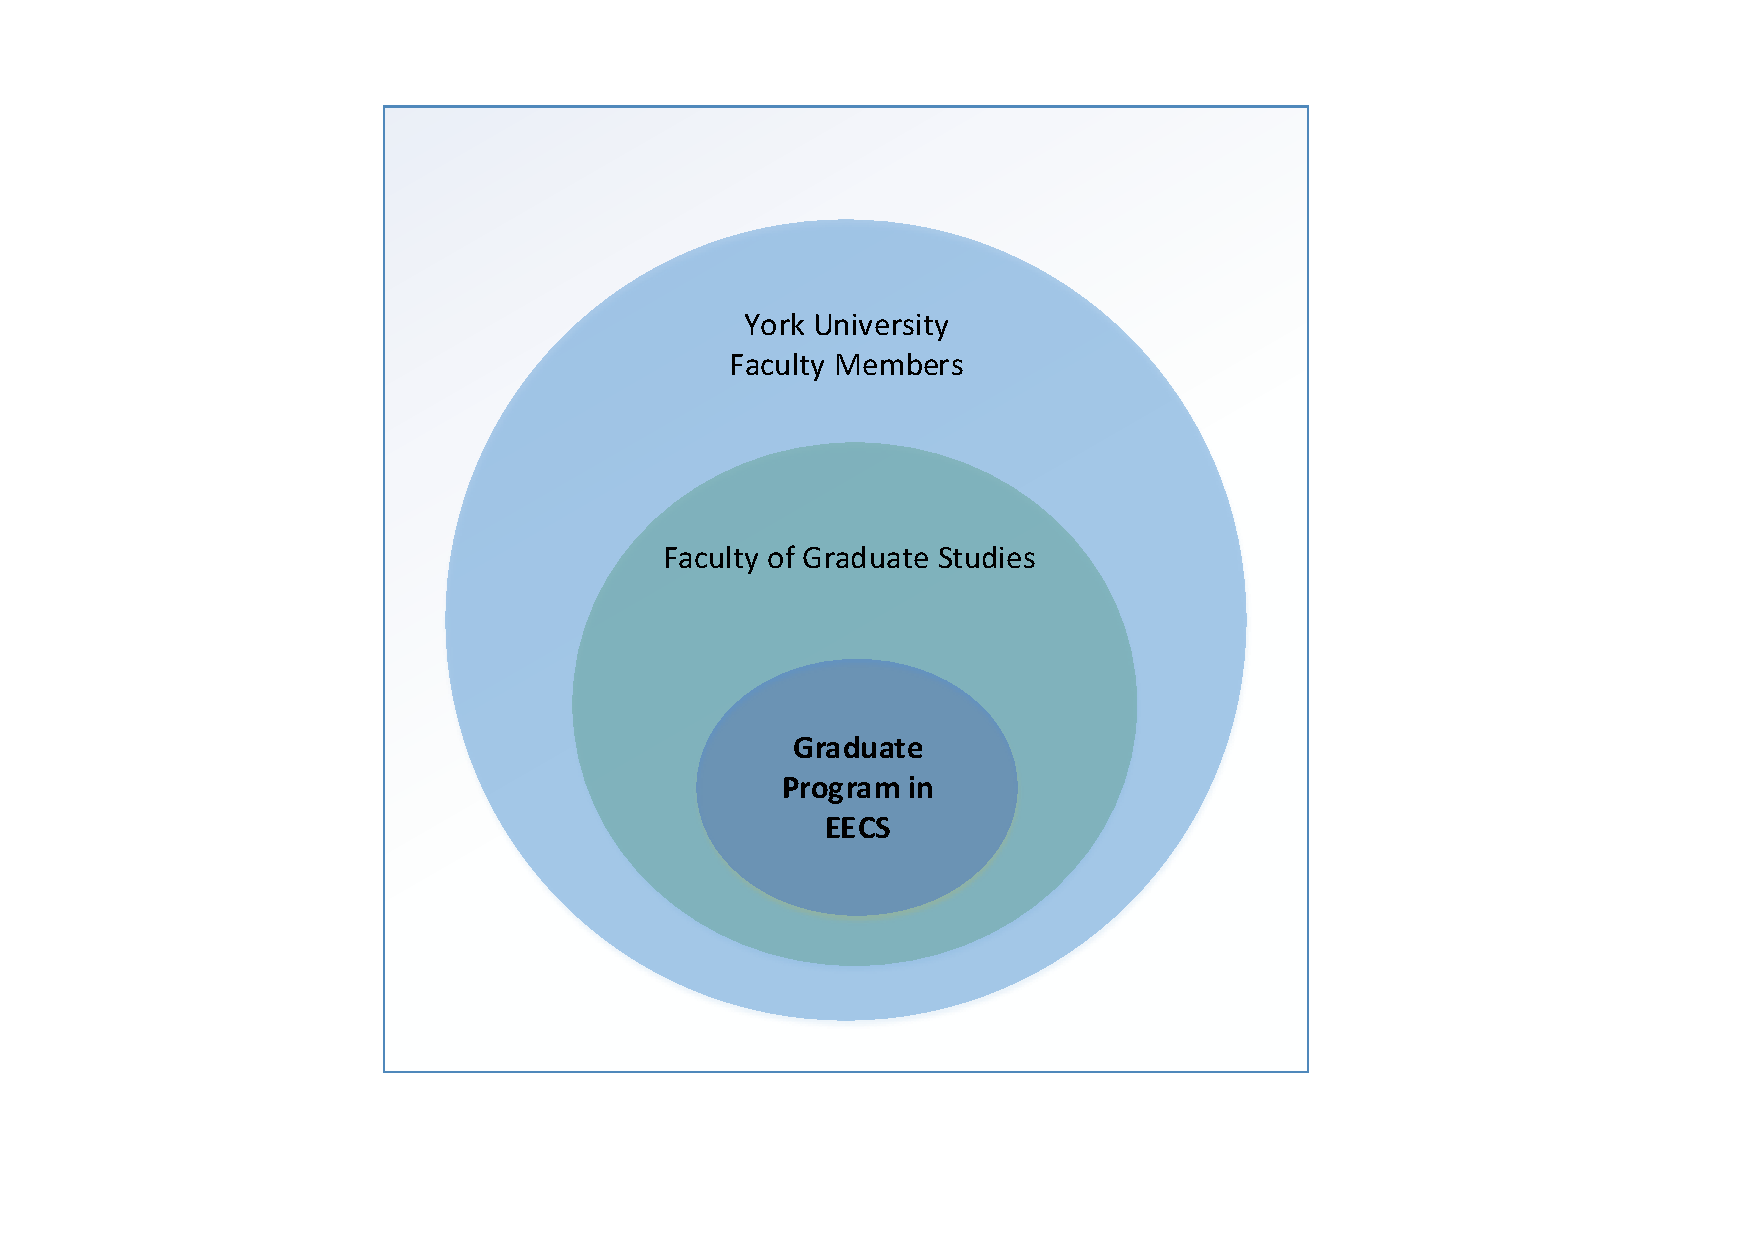
\includegraphics[width=.65\textwidth]{images/faculty_venn_diagram.pdf}
\end{center}
\caption{Faculty Members Venn Diagram}
\label{fig:faculty_venn_diagram}
\end{figure}

\newpage
\section{System Goals}

The current system in place for the the EECS Graduate Program completes the bare minimum requirement of displaying student applications to professors. However, faculty members express their frustration about the amount of time that is required to find a suitable graduate student ranging from uploading a student application to requesting a student for admission.

\bigskip

\noindent As a result we have set the following high-level goals (\textbf{G}) to reduce frustration and improve efficiency:

\smallskip

\begin{mylist}

\item \textbf{G1}---An Admin should be able to add/remove/modify student applications in the system.

\item \textbf{G2}---An Admin should be able to assign applications to be reviewed by Committee Members.

\item \textbf{G3}---An Admin should be able to manage Committee Members.

\item \textbf{G4}-- An Admin should be able to assign/remove roles of other faculty members.

\item \textbf{G5}---A Committee Member should be able to view applications to be reviewed.

\item \textbf{G6}---A Committee Member should be able to use/modify/add university descriptions in the system for their reviews.

\item \textbf{G7}---A Professor and Admin should be able to search for desired student applications by applying a filter (See Appendix \ref{app:defns}) on application attributes.

\item \textbf{G8}---A Professor should be able to indicate Admins to request a student for admission.
\end{mylist}


\newpage
\section{Set Dictionary}

The following table denotes a set dictionary describing the mathematical sets defined in the system:

\begin{table}[!htb]
\begin{tabular}{| c | c | c |}
	\cline{1-3}
	\textbf{Set} & \textbf{Notation} & \textbf{Description} \\ \hline
	$STAFF$ & & Set of all staffs \\
	& & at York University\\ \hline
	$FM$ & $FM \subseteq STAFF$ & Set of all faculty members \\
	& & in the EECS graduate\\
	& & program \\ \hline
	$APPS$ & & Set of all student applications\\
	& & in the EECS graduate \\
	& & program \\ \hline
	$ADMIN$ & $ADMIN \subseteq FM$ & Set of all admins \\ \hline
	$GPA$ & ($GPA \subseteq STAFF)$ & Grad Program Assistant \\
	& $\land$ & in the EECS graduate \\
	& $(GPA \neq FM)$ & program \\ \hline
	$GC$ & $GC \subseteq FM$  & Set of all graduate \\
	& & committee members\\ \hline
	$PROF$ & $PROF \subseteq FM$ & Set of all professors \\ \hline 
	$UPLOADED$ & $UPLOADED \subseteq APPS$ & Set of all uploaded \\
	& & applications \\ \hline
	$ASSIGNED$ & $ASSIGNED \subseteq APPS$ & Set of all assigned \\
	& & applications \\ \hline
	$REVIEWED$ & $REVIEWED \subseteq APPS$ & Set of all reviewed \\
	& & applications \\ \hline
	$TBR$ & $TBR \subseteq ASSIGNED$ & Set of all to \\
	& & be reviewed applications \\ \hline
	$IN\_PROGRESS$ & $IN\_PROGRESS \subseteq$ & Set of all applications \\
	& $(ASSIGNED \setminus TBR)$ & in progress \\ \hline
	$DRAFT$ & $DRAFT \subseteq IN\_PROGRESS$ & Set of all applications \\
	& & saved as draft\\ \hline
	$ATTR$ & Refer to table: \ref{tbl:attr_uploaded} and \ref{tbl:attr_reviewed} & Set of all application \\
	& & attributes\\ \hline
	$APP\_STATUS$ & $APP\_STATUS \subseteq$  & Set of all application \\
	& $(ATTR = "Application Status")$ & status\\ \hline
	$REV\_STATUS$ & $REV\_STATUS \subseteq$  & Set of all review status\\ 
	& $(ATTR = "Review Status")$ & \\ \hline
\end{tabular}
\caption {Description table for mathematical sets used in the System Under Description}
\label{tbl:sets1}
\end{table}

\newpage
\section{Roles} \label{roles}

The \textbf{three} major roles in our business system are: \emph{administrator}, \emph{committee member} and \emph{professor}. In other words, a faculty member, $fm$, such that $fm \in FM$ needs to have at least one role assigned to them in order to access the system. The diagram Fig.~\ref{fig:all_roles_sud} depicts the roles along with descriptions in each subsection:

\begin{figure}[!htb]
\begin{center}
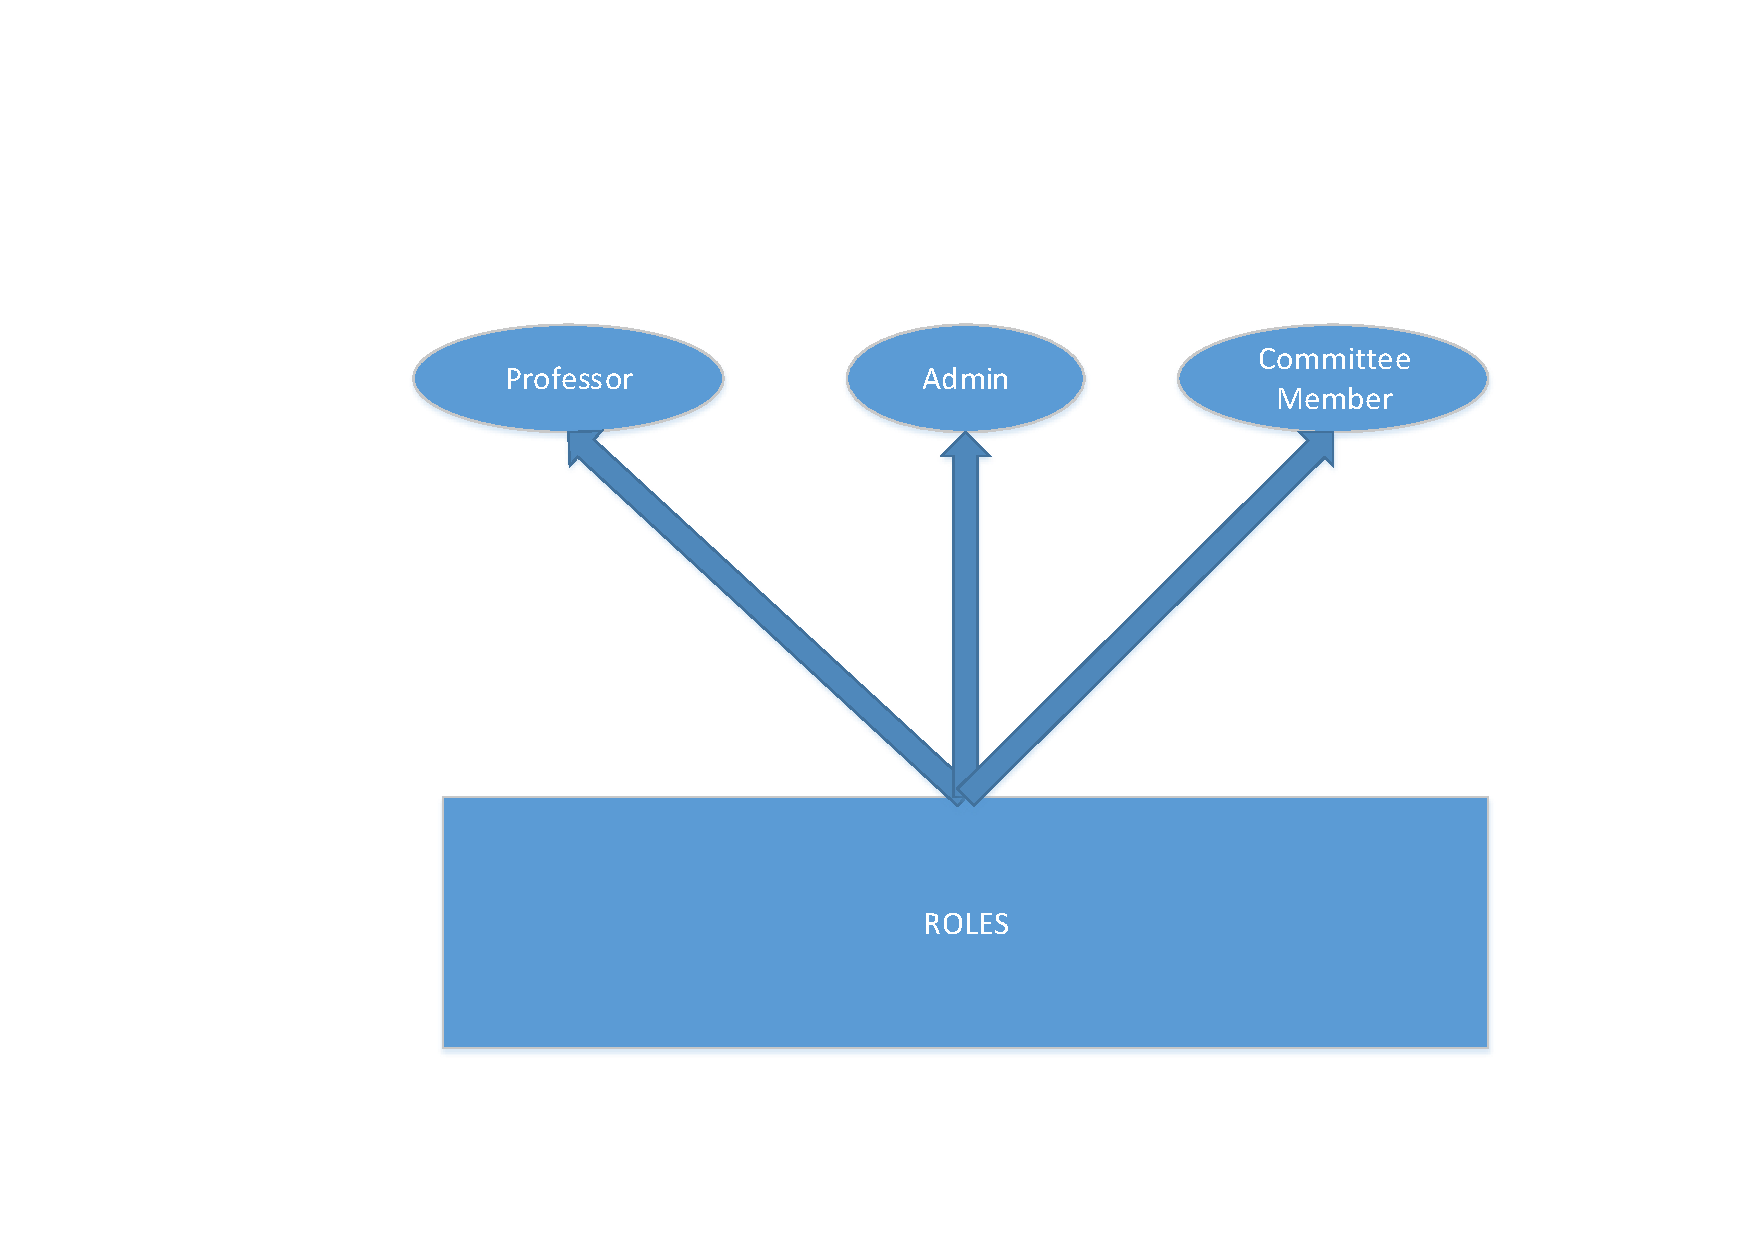
\includegraphics[width=.8\textwidth]{images/all_roles.pdf}
\end{center}
\caption{Roles in System Under Description}
\label{fig:all_roles_sud}
\end{figure}

\subsection{Admin}

The \emph{admin} in our system under description are  the \emph{Graduate Program Director (GPD)} and the \emph{Graduate Program Assistant (GPA)}. The GPA is an \textbf{exception} case for an Admin despite not being a member of the graduate program refer to Table \ref{tbl:sets1}. The admins have the master control of the overall system starting from adding/removing graduate program members into the system to sending out the final decision for an applicant. A breakdown of an \emph{admin's} permissible actions are listed below.

\smallskip
\noindent An \emph{admin}:

\begin{mylist}
\item Can add a new member to the list of EECS graduate program members
\item Can remove a member from the list of EECS graduate program members except for themselves
\item Can assign a new role to an existing member
\item Can assign applications to be reviewed by a graduate committee member
\item Can send email reminders to committee members about assigned applications
\item Can upload a student application to the portal
\item Can update all attributes of a student application
\end{mylist}

\subsection{Committee Member}

The \emph{committee member} in our system under description is a subset of EECS graduate program members who are in charge of reviewing new applications. The role of a graduate committee member, $gcm$, such that $gcm \in GC$, is to review the student application(s) that are assigned to them by an \emph{admin}. A breakdown of a \emph{committee member's} permissible actions are listed below.

\smallskip
\noindent A \emph{committee member}:

\begin{mylist}
\item Can review an assigned application(s)
\item Can view past reviewed application(s)
\item Can add/use/modify university descriptions in the system to be used for all applications.
\end{mylist}

\subsection{Professor}

The \emph{professors} in our system are a subset of EECS graduate program members who are in charge of choosing a student once the final application with reviews have been uploaded to the portal. The role of a professor, $prof$, such that $prof \in PROF$, is to select a student who is interested in their field of studies satisfying the admission requirements. Once a professor is interested in a student, they can contact the student as well as request the student for admission to the \emph{admin}. A breakdown of a \emph{professor's} permissible actions are listed below.

\smallskip
\noindent A \emph{professor}:

\begin{mylist}
\item Can contact a student, once interested
\item Can request a student for admission, once	 contacted
\end{mylist}

\newpage
\section{Deliverables}

The deliverables for this project upon reaching an agreement with our clients were broken into two parts: \textbf{Required} \ref{req_delvs} and \textbf{Optional} \ref{opt_delvs}.

\smallskip

\noindent The \emph{Required} deliverables are required to have fully functional services and on the other hand, \emph{Optional} deliverables are optional services that could be achieved if and only if all the required deliverables have been completed.

\subsection{Required Deliverables} \label{req_delvs}

The \emph{Required} deliverables were decided by the majority vote on a list of questionnaires conducted on the EECS graduate program members. Following are the \textbf{\emph{Required}} deliverables for the System Under Description:\\

\begin{mylist}
\item Any user shall be able to log into the system if and only if they are a member of the EECS graduate program
\item Any user shall be able to log out of the system if and only if they are logged in
\item Any user shall be logged out of the system after a maximum of 15 minutes of idleness
\item An \emph{admin} shall be able to add a new member to the list of EECS graduate program members
\item An \emph{admin} shall be able to remove a member from the list of EECS graduate program members except for themselves
\item An \emph{admin} shall be able to assign a new role to an existing faculty member
\item An \emph{admin} shall be able to assign applications to be reviewed by committee members
\item An \emph{admin} shall be able to upload a student application to the portal
\item An \emph{admin} shall be able to update all attributes of a student application
\item An \emph{admin} who assigned an application shall be notified when reviews for that application has been completed
\item An \emph{admin} shall be able to export the applications to CSV format
\item A \emph{committee member} shall be notified when a batch of applications come in for review
\item A \emph{committee member} shall be able to see the list of new and previously reviewed application(s)
\item A \emph{committee member} shall be able to apply filtering only on previously reviewed application(s)
\item A \emph{committee member} shall be able to save applications as a draft for future completion
\item A \emph{committee member} shall be able to view, use or modify a university assessment if it has already been used when reviewing applications
\item An \emph{admin} and \emph{professor} shall be able to see details about an application in an organized table with the following attributes:
\begin{enumerate}
\item Date of Application
\item Year
\item Session
\begin{enumerate}
\item Fall
\item Winter
\item Summer
\end{enumerate}
\item Student ID
\item Name
\item Gender
\begin{enumerate}
\item M
\item F
\end{enumerate}
\item Field of Interest(s)
\begin{enumerate}
\item Artificial Intelligence
\item Bioinformatics
\item Biomedical Engineering
\item Computational Neuroscience
\item Computational Biology
\item Computer Graphics and Media
\item Computer Security and Networks
\item Computer Vision
\item Data Science
\item Data Mining
\item Distributed Computing
\item Embedded Systems
\item History of Computing
\item Human-Computer Interaction
\item Graph Mining
\item Integrated Circuits and Systems
\item Large-scale Software Systems
\item Micro/Nano Electronic Systems
\item Machine Learning
\item Performance Engineering
\item Power and Renewable Energy Systems
\item Robotics
\item Signal Processing
\item Software Engineering
\item Theory of Computation
\end{enumerate}
\item Preferred Professor(s)
\begin{enumerate}
\item Provide with list of the members of the EECS graduate program
\end{enumerate}
\item Committee Ranking
\begin{enumerate}
\item A+ (definite admit)
\item A (likely admit)
\item B+ (possible admit)
\item B (reserve list)
\item C (reject)
\end{enumerate}
\item GPA
\item Degree Applied For
\begin{enumerate}
\item MSc
\item MASc
\item PhD
\end{enumerate}
\item Visa Status
\begin{enumerate}
\item Visa
\item Domestic
\end{enumerate}
\item Committee Reviewer
\begin{enumerate}
\item Provide with list of the members of the EECS graduate program who are in the graduate committee
\end{enumerate}
\item Application Status
\begin{enumerate}
\item Contacted by *Professor* - once the student has been contacted by one or more professor
\item Requested by *Professor* - once the student has been requested by one or more professor
\item Decision by Program
\begin{enumerate} 
\item Accepted
\item Declined
\item No Decision Made Yet
\end{enumerate}
\item Decision by Student
\begin{enumerate}
\item Accepted
\item Declined
\item No Decision Made Yet
\end{enumerate}
\item Date letter sent
\item YGS Awarded
\item Reason for Decline
\item Comment
\end{enumerate}
\item Reviewed Status (Similar to application status but is user specific)
\begin{enumerate}
\item Reviewed - once a professor has seen a student application and decided to not move on to contact them
\item Not Reviewed - not looked into the application yet
\end{enumerate}
\end{enumerate}
\item An \emph{admin} and \emph{professor} shall be able to perform advanced filtering on all of the above attributes
\item In addition, \emph{Application Status} attribute can only be filtered on:
\begin{enumerate}
\item The date of application uploaded
\item The professor(s) who has been in contact with the student
\item The professor(s) who has requested the student
\item The decision by the program
\item The decision by the student
\end{enumerate}
\end{mylist}

\smallskip
\noindent \textbf{Rationale on Field of Interest(s)}: The initial field of interest(s) had too much overlapping between fields. After conducting a questionnaire on the graduate program members, we came up with a much more distinguished set of field interest(s). Some of the changes from the initial list were:
\begin{mylist}
\item Adding important fields that were missing, e.g
\begin{enumerate}
\item Data Mining
\item Embedded Systems
\item Machine Learning
\item Software Engineering
\end{enumerate}
\item Combine fields that has the same set of researchers into one, e.g
\begin{enumerate}
\item Merge Big Data and Information Systems into just Data Science
\item Merge Adaptive Systems into just Artificial Intelligence
\end{enumerate}
\item Separate fields that have too much overlapping into two different fields, e.g
\begin{enumerate}
\item Computer Vision and Robotics were broken down into two fields
\begin{enumerate}
\item Computer Vision
\item Robotics
\end{enumerate}
\end{enumerate}
\end{mylist}

\bigskip

\noindent\textbf{Application Attributes}

\smallskip

\noindent An \emph{admin} or a \emph{professor}, can see a list of student applications once uploaded to the system and a review has been completed. The following table denotes the attributes of a student application:

\begin{table}[!htb]
\begin{tabular}{| c | c | c |}
	\cline{1-3}
	\textbf{Attribute} & \textbf{Type} & \textbf{Range}\\ \hline
	Date of Application & Date & \\ \hline
	Year & Int & $0000 ... 9999$ \\ \hline
	Session & Enumerated & $\{Fall, Winter, Summer\}$ \\ \hline
	Student ID & Big Int & $000000000 ... 999999999$ \\ \hline
	Name & String & \\ \hline
	Gender & Enumerated & $\{M, F\}$ \\ \hline
	Field of Interest(s) & Enumerated & Refer to Section \ref{req_delvs} \\ \hline
	Preferred Professor(s) & Enumerated & $FM$ \\ \hline
	Committee Ranking & Enumerated & $\{A+, A, B+, B, C\}$ \\ \hline
	GPA & Any & \\ \hline
	Degree Applied For & Enumerated & $\{MSc, MASc, PhD\}$ \\ \hline
	Visa Status & Enumerated & $\{Visa, Domestic\}$ \\ \hline
	Committee Reviewer & Enumerated & $GC$ \\ \hline
	Application Status & Enumerated & Refer to Section \ref{req_delvs} \\ \hline
	Reviewed Status & Enumerated & $\{Reviewed, Not Reviewed\}$ \\ \hline
\end{tabular}
\caption {Attributes on uploaded applications}
\label{tbl:attr_uploaded}
\end{table}


\noindent A \emph{committee member}, can see a list of student applications due for review or previously reviewed applications. The following table denotes the attributes of a reviewed student application:

\begin{table}[!htb]
\begin{tabular}{| c | c | c |}
	\cline{1-3}
	\textbf{Attribute} & \textbf{Type} & \textbf{Range}\\ \hline
	Date of Application & Date & \\ \hline
	Student ID & Big Int & $000000000 ... 999999999$ \\ \hline
	Application Status & Enumerated & $\{Reviewed, Not Reviewed, Draft Available\}$ \\ \hline
\end{tabular}
\caption {Attributes on uploaded applications}
\label{tbl:attr_reviewed}
\end{table}

\noindent \textbf{\\Rationale on initial attributes}: On the grad apps webpage, the system should be listing the \textbf{top 7} attributes that were voted for when seeing the application. This to ensure a reasonable amount of information about an application is contained initially to view an application. With the use of filtering, one can always see more or less fields than the initial view.

\newpage
\subsection{Optional Deliverables} \label{opt_delvs}

The \emph{Optional} deliverables were decided by the minority vote on a list of questionnaires conducted on the EECS graduate program staffs. Following are the \textbf{\emph{Optional}} deliverables for the System Under Description:\\

\begin{mylist}
\item An \emph{admin} may be able to import a CSV file and extend the database with the new data
\item A \emph{committee member} completing a review form may be able to have a head start on the form with information automatically extracted and filled such as Name, Student No., GPA
\item A \emph{committee member} may be able to download offline forms (XML format) and upload it back into the server
\item A \emph{professor} might be interested in other attributes that are to be provided in an organized table and used for advanced filtering
\begin{enumerate}
\item Previous University
\item GRE
\item Other English proficiency test scores
\begin{enumerate}
\item IELTS
\item TOEFL
\item YELT
\end{enumerate}
\end{enumerate}
\item A \emph{professor} may be able to contact students on behalf of a research group (i.e instead of multiple professor from the same field contacting a student, they might want to contact the student as part of a group eg. vision, databases, etc.)
\item A \emph{professor} may be able to contact student (email) directly from the application
\item A \emph{professor} may be able to leave notes on an application for personal use or for other professors to view when going through the same application
\end{mylist}

\newpage
\section{System Invariants}	\label{sec:invs}

\geninv{There must be at least one admin in the system.}{}\label{INV1}
\geninv{User private attributes such as reviewed status and drafted applications can only be used by that user.}{}\label{INV2}
\geninv{Committee members only have access to the applications assigned to them.}{}\label{INV3}
\geninv{An application must be reviewed before Professors can access them.}{}\label{INV4}
\geninv{A user must be logged in with exactly one role.}{}\label{INV5}

%%%%%%%%%%%%%%%%%%%%%%%%%%%%%%%%%%%%%%%%%%%%%%%%%%%%%%%%%%%%%%%%%%%%%%%%
\newpage
\section{Use Case Diagram} \label{sec:ucd}

The following is an abstract Use Case Diagram for the System Under Description. The actors in the Use Case Diagram are the: \emph{admin}, \emph{professor} and \emph{committee member} as discussed in Section \ref{roles}.

\begin{figure}[!htb]
\begin{center}
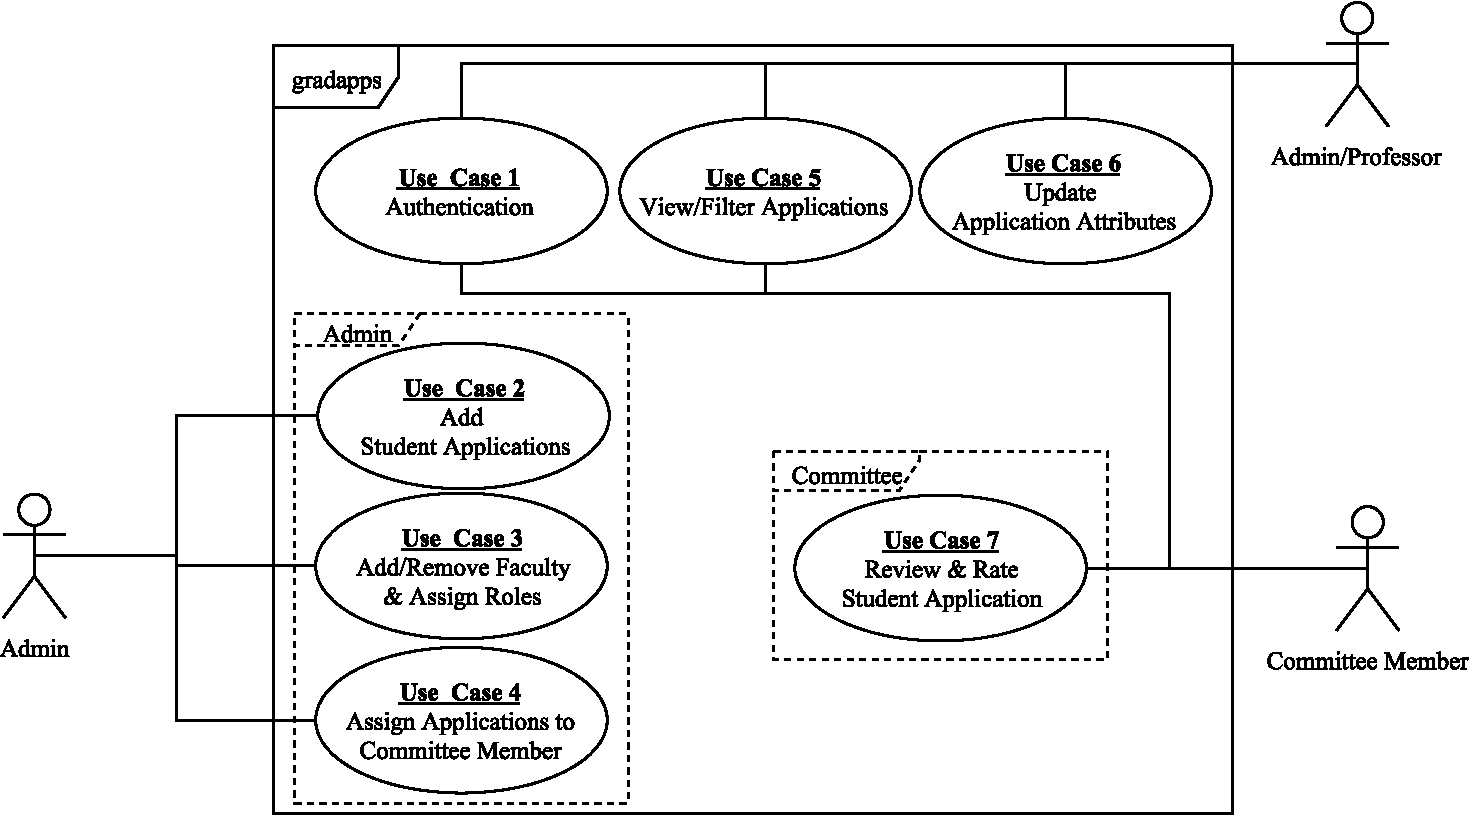
\includegraphics[width=.99\textwidth]{images/gradapps-usecase.pdf}
\end{center}
\caption{Use Case Diagram for the System Under Description}
\label{fig:ucd}
\end{figure}

\newpage
\section{Use Case Textual Description} \label{sec:uctd}

The following are the Use Case Textual Description for the diagram provided in Section \ref{sec:ucd}. A list of success and error messages are provided in Appendix \ref{app:success} and \ref{app:error} respectively.
\newpage
\subsection{Use Case 1 - Authentication} \label{subsec:uc1}

The following three use case textual representation describes the \emph{Authentication} use case.


\begin{itemize}
\item Table \ref{tbl:uc1Atd} describes a user is logging into the system
\item Table \ref{tbl:uc1Btd} describes a user once validated, selecting a role to log in as.
\item Table \ref{tbl:uc1Ctd} describes a user logging out of the system.
\end{itemize}

\begin{table}[!htb]
\begin{center}
\begin{tabular}{|l|l|}
\hline
\textbf{Use Case ID:} UC-1A \\ \hline
\textbf{Use Case Name:} Login \\ \hline
\textbf {Primary Actor:} Admin, Professor, Committee Member\\ \hline
\textbf{Description:} A user opens the browser and goes to the portal webpage. \\The user enters their Passport York username along with the password associated \\with it. The user clicks the login button, the credentials get authenticated \\and succeeds. The user is now logged into the system. \\ \hline
\textbf{Trigger:} User indicates to login to the system.\\ \hline
\textbf{Precondition:}
\\ PRE-1. The user has a PPY account. 
\\ PRE-2. The user is not logged into the system. \\ \hline
\textbf{Postcondition:}
\\ POST-1. The user is logged into the system. \\ \hline
\textbf{Normal Flow: 1A.0 Login to the system}
\\ 1. User opens a web browser and visits the grad apps webpage.
\\ 2. System prompts the user to enter their PPY username and password.
\\ 3. User enters the username and password and clicks enter.
\\ 4. System sends authentication request to PPY and gets a valid response back.
\\ 5. The user is redirected to the next page for selecting the role. Extension \\point to UC-3.\\ \hline
\textbf{Exception Flow: 1A.0.E1 User ID or Password is not valid}
\\ 1. System displays error \hyperref[app:error]{\textbf{e1}}
\\ 2. System awaits for the user to re-enter a correct ID and password \\(3a) or to exit (3b).
\\ 3a. System starts normal flow over.
\\ 3b. System terminates the use case.\\ \hline
\end{tabular}
\end{center}
\caption {Use Case Textual Description for Login}
\label{tbl:uc1Atd}
\end{table}

\begin{table}[!htb]
\begin{center}
\begin{tabular}{|l|l|}
\hline
\textbf{Use Case ID:} UC-1B \\ \hline
\textbf{Use Case Name:} Select Role \\ \hline
\textbf {Primary Actor:} Admin, Professor, Committee Member\\ \hline
\textbf{Description:} A user has logged into the system. A prompt is shown \\to the user to select a role they are assigned to. The user selects \\one of the roles and proceeds into the next page.\\ \hline
\textbf{Precondition:}
\\ PRE-1. The user is logged in to the system. \\ \hline
\textbf{Postcondition:}
\\ POST-1. The user logs in with the selected a role. \\ \hline
\textbf{Normal Flow: 1B.0 Select Role}
\\ 1. User selects the role they want to use the system with.
\\ 2. System prompts the user to confirm the selection of the role.
\\ 3. User chooses yes.
\\ 4. System requests all access for the user in the role and succeeds.
\\ 5. The user is now able to access the system with a particular role.\\ \hline
\textbf{Exception Flow: 1B.0.E1 Role selected is invalid}
\\ 1. System displays error \hyperref[app:error]{\textbf{e2}}.
\\ 2. System awaits for the user to select another role \\(3a) or to exit (3b).
\\ 3a. System starts normal flow over.
\\ 3b. System terminates the use case.\\ \hline
\end{tabular}
\end{center}
\caption {Use Case Textual Description for Role Selection}
\label{tbl:uc1Btd}
\end{table}

\begin{table}[!htb]
\begin{center}
\begin{tabular}{|l|l|}
\hline
\textbf{Use Case ID:} UC-1C \\ \hline
\textbf{Use Case Name:} Logout \\ \hline
\textbf {Primary Actor:} Admin, Professor, Committee Member\\ \hline
\textbf{Description:} A user is already logged into the system. The user clicks on the \\logout button. The user's logged in session is successfully terminated by PPY \\and the user is bought back into the login page. \\ \hline
\textbf{Trigger:} User indicates to logout of the system.\\ \hline
\textbf{Precondition:}
\\ PRE-1. The user is logged in to the system.
\\ PRE-2. The user has a selected role. \\ \hline
\textbf{Postcondition:}
\\ POST-1. The user is logged out of the system. \\ \hline
\textbf{Normal Flow: 1C.0 Logout of the system}
\\ 1. User clicks on the logout button.
\\ 2. System prompts the user to confirm logging out of the system.
\\ 3. User chooses ok.
\\ 4. System sends session termination request to PPY and gets a valid response back.
\\ 5. The user is logged out and redirected to the login page.\\ \hline
\textbf{Exception Flow: 1C.0.E1 Already logged out}
\\ 1. System displays error \hyperref[app:error]{\textbf{e3}}
\\ 2. User is redirected to the login pages
\\ 3. System terminates the use case.\\ \hline
\end{tabular}
\end{center}
\caption {Use Case Textual Description for Logout}
\label{tbl:uc1Ctd}
\end{table}

\clearpage
\newpage
\subsection{Use Case 2 - Add Student Application} \label{subsec:uc2}
\begin{table}[!htb]
\begin{center}
\begin{tabular}{|l|l|}
\hline
\textbf{Use Case ID:} UC-2 \\ \hline
\textbf{Use Case Name:} Add Student Application \\ \hline
\textbf {Primary Actor:} Admin \\ \hline
\textbf{Description:} A user has logged into the system. The user wants to \\add an application to the system. The user selects the option to add \\an application, a prompt is shown to enter the details about the application \\and select a PDF formatted file of the application. The user enters the information \\and submits a request. The system confirms success in uploading the application.\\ \hline
\textbf{Trigger:} User indicates to add an application to the system.\\ \hline
\textbf{Precondition:}
\\ PRE-1. The user is logged in. 
\\ PRE-2. The role selected by the user is admin. \\ \hline
\textbf{Postcondition:}
\\ POST-1. The user has added an application to the system. \\ \hline
\textbf{Normal Flow: 2.0 Add a Student Application}
\\ 1. User selects the option to add an application.
\\ 2. System prompts the user to enter details about the application and \\select a PDF file.
\\ 3. User enters the information and clicks enter.
\\ 4. System validates the information provided and succeeds.
\\ 5. The user is shown success message \hyperref[app:success]{\textbf{s5}}.
\\ \hline
\textbf{Exception Flow: 2.0.E1 File uploaded is not of the correct type}
\\ 1. System displays error \hyperref[app:error]{\textbf{e9}}.
\\ 2. System prompts the user to try uploading file of PDF type (3a) or to exit (3b). \\ \hline 
\textbf{Exception Flow: 2.0.E2 Incorrect type of value entered}
\\ 1. System displays error  \hyperref[app:error]{\textbf{e10}}.
\\ 2. System awaits for the user to re-enter a new value (3a) or to exit (3b). \\ \hline 
\textbf{Exception Flow: 2.0.E3 Not an Admin}
\\ 1. System displays error  \hyperref[app:error]{\textbf{e12}}.
\\ 2. System exits (3b). \\ \hline 
\textbf{Exception Flow}
\\ 3a. User requests to try again. System starts normal flow over.
\\ 3b. User asks to exit. System terminates the use case.
\\ \hline
\end{tabular}
\end{center}
\caption {Use Case Textual Description for Adding an Application}
\label{tbl:uc2td}
\end{table}

\clearpage
\newpage
\subsection{Use Case 3 - Add/Remove Members and Assign Roles} \label{subsec:uc3}

The following four use case textual representation describes the \emph{Add/Remove Members and Assign Roles} use case.

\begin{itemize}
\item Table \ref{tbl:uc3Atd} describes adding a new faculty member to the system.
\item Table \ref{tbl:uc3Btd} describes removing a faculty member from the system.
\item Table \ref{tbl:uc3Ctd} describes assigning a role to a faculty member in the system.
\item Table \ref{tbl:uc3Dtd} describes unassigning a role from a faculty member in the system.
\end{itemize}

\begin{table}[!htb]
\begin{center}
\begin{tabular}{|l|l|}
\hline
\textbf{Use Case ID:} UC-3A \\ \hline
\textbf{Use Case Name:} Add a Member \\ \hline
\textbf {Primary Actor:} Admin \\ \hline
\textbf{Description:} A user has logged into the system. \\The user wants to add a new user. The user selects the option to \\add a new member, a prompt is shown to enter the member's PPY id. \\ The user enters all the information and submits a request. \\ The system confirms success in adding the new member.\\ \hline
\textbf{Precondition:}
\\ PRE-1. The user is logged in.
\\ PRE-2. The role selected by the user is admin.
\\ PRE-3. The member to be added is not in the system. \\ \hline
\textbf{Postcondition:}
\\ POST-1. The member has been added to the system. \\ \hline
\textbf{Normal Flow: 3A.0 Add a new member}
\\ 1. User selects the option to add a new member.
\\ 2. System prompts the user to enter the member ID.
\\ 3. User enters the information and clicks enter.
\\ 4. System validates the information provided and succeeds.
\\ 5. The user is shown a success message \hyperref[app:success]{\textbf{s1}}.\\ \hline
\textbf{Exception Flow: 3A.0.E1 Member with the ID does not exist}
\\ 1. System displays error \hyperref[app:error]{\textbf{e4}}.
\\ 2. System prompts the user to try adding another member (3a) or to exit (3b). \\ \hline
\textbf{Exception Flow: 3A.0.E2 Not an Admin}
\\ 1. System displays error  \hyperref[app:error]{\textbf{e12}}.
\\ 2. System exits (3b). \\ \hline 
\textbf{Exception Flow}
\\ 3a. User requests to add another member. System starts normal flow over
\\ 3b. User asks to exit. System terminates the use case.\\ \hline

\end{tabular}
\end{center}
\caption {Use Case Textual Description for Add a New Member}
\label{tbl:uc3Atd}
\end{table}

\begin{table}[!htb]
\begin{center}
\begin{tabular}{|l|l|}
\hline
\textbf{Use Case ID:} UC-3B \\ \hline
\textbf{Use Case Name:} Remove a Member \\ \hline
\textbf {Primary Actor:} Admin \\ \hline
\textbf{Description:} A user has logged into the system. The user wants to remove\\ a user from the system. The user selects the option to remove the member,\\ a prompt is shown to enter the member's PPY id. \\The user enters all the information and submits a request. \\The system confirms success in removing the member.\\ \hline
\textbf{Precondition:}
\\ PRE-1. The user is logged in.
\\ PRE-2. The role selected by the user is admin.
\\ PRE-3. The member to be removed is in the system. \\ \hline
\textbf{Postcondition:}
\\ POST-1. The member is removed from the system. 
\\ POST-2. The member is logged out if logged in.\\ \hline
\textbf{Normal Flow: 3B.0 Remove an existing member}
\\ 1. User selects the option to remove an existing member.
\\ 2. System prompts the user to enter the member ID.
\\ 3. User enters the information and clicks enter.
\\ 4. System validates the information provided and succeeds.
\\ 5. The user is shown a success message \hyperref[app:success]{\textbf{s2}}.
.\\ \hline
\textbf{Exception Flow: 3B.0.E1 Member with the ID does not exist}
\\ 1. System displays error \hyperref[app:error]{\textbf{e5}}.
\\ 2. System prompts the user to try removing another member (3a) or to exit (3b).
\\ \hline
\textbf{Exception Flow: 3B.0.E2 Not an Admin}
\\ 1. System displays error  \hyperref[app:error]{\textbf{e12}}.
\\ 2. System exits (3b). \\ \hline 
\textbf{Exception Flow}
\\ 3a. User requests to remove another member. System starts normal flow over
\\ 3b. User asks to exit. System terminates the use case.\\ \hline
\end{tabular}
\end{center}
\caption {Use Case Textual Description for Remove an Existing Member}
\label{tbl:uc3Btd}
\end{table}


\begin{table}[!htb]
\begin{center}
\begin{tabular}{|l|l|}
\hline
\textbf{Use Case ID:} UC-3C \\ \hline
\textbf{Use Case Name:} Assign a Role \\ \hline
\textbf {Primary Actor:} Admin \\ \hline
\textbf{Description:} A user has logged into the system. The user wants to assign \\a new role to an existing user. \\The user selects the option to assign the role of a member, a prompt is shown \\to enter the member's PPY id and the role to be assigned. The user enters \\the information and submits a request. The system confirms success in \\adding the members role.\\ \hline
\textbf{Precondition:}
\\ PRE-1. The user is logged in.
\\ PRE-2. The role selected by the user is admin.
\\ PRE-3. The member is in the system.
\\ PRE-4. The role to be assigned is a valid role. Refer to Section \ref{roles}. \\ \hline
\textbf{Postcondition:}
\\ POST-1. The member has a new role associated. \\ \hline
\textbf{Normal Flow: 3C.0 Assign a new role to an existing member}
\\ 1. User selects the option to assign a new role to an existing member.
\\ 2. System prompts the user to enter the member ID and the role to be assigned.
\\ 3. User enters the information and clicks enter.
\\ 4. System validates the information provided and succeeds.
\\ 5. The user is shown a success message \hyperref[app:success]{\textbf{s3}}.
\\ \hline
\textbf{Exception Flow: 3C.0.E1 Member with the ID does not exist}
\\ 1. System displays error \hyperref[app:error]{\textbf{e5}}.
\\ 2. System prompts the user to try again on another member (3a) or exit (3b).
\\ \hline
\textbf{Exception Flow: 3C.0.E2 Member already has the role assigned}
\\ 1. System displays error \hyperref[app:error]{\textbf{e6}}.
\\ 2. System prompts the user to try again on another member (3a) or exit (3b).
\\ \hline
\textbf{Exception Flow: 3C.0.E3 Not an Admin}
\\ 1. System displays error  \hyperref[app:error]{\textbf{e12}}.
\\ 2. System exits (3b). \\ \hline 
\textbf{Exception Flow: 3C.0.E4 Role is invalid} 
\\ 1. System displays error  \hyperref[app:error]{\textbf{e13}}.
\\ 2. System prompts the user to try again on another member (3a) or exit (3b). \\ \hline 
\textbf{Exception Flow}
\\ 3a. User requests to assign a role to another member. \\System starts normal flow over
\\ 3b. User asks to exit. System terminates the use case.\\ \hline
\end{tabular}
\end{center}
\caption {Use Case Textual Description for Assign a New Role}
\label{tbl:uc3Ctd}
\end{table}

\begin{table}[!htb]
\begin{center}
\begin{tabular}{|l|l|}
\hline
\textbf{Use Case ID:} UC-3D \\ \hline
\textbf{Use Case Name:} Unassign a Role \\ \hline
\textbf {Primary Actor:} Admin \\ \hline
\textbf{Description:} A user has logged into the system. The user wants to \\unassign a role for an existing user. \\The user selects the option to unassign the role of a member, a prompt is \\shown to enter the member's PPY id and the role to be unassigned. The user \\enters the information and submits a request. The system confirms success in \\removing the members role.\\ \hline
\textbf{Precondition:}
\\ PRE-1. The user is logged in.
\\ PRE-2. The role selected by the user is admin.
\\ PRE-3. The member is in the system.
\\ PRE-4. The member is assigned the role to be removed. \\ \hline
\textbf{Postcondition:}
\\ POST-1. The member is not associated to the role.
\\ POST-2. The member is logged out if using the role removed. \\ \hline
\textbf{Normal Flow: 3D.0 Unassign a role from an existing member}
\\ 1. User selects the option to unassign a role of an existing member.
\\ 2. System prompts the admin to enter the member ID and 
\\ the role to be unassigned.user
\\ 3. User enters the information and clicks enter.
\\ 4. System validates the information provided and succeeds.
\\ 5. The user is shown a success message \hyperref[app:success]{\textbf{s4}}.
\\ \hline
\textbf{Exception Flow: 3D.0.E1 Member with the ID does not exist}
\\ 1. System displays error \hyperref[app:error]{\textbf{e5}}.
\\ 2. System prompts the user to try again on member (3a) or to exit (3b).
\\ \hline
\textbf{Exception Flow: 3D.0.E2 Member already has the role assigned}
\\ 1. System displays error \hyperref[app:error]{\textbf{e6}}.
\\ 2. System prompts the user to try again on another member (3a) or to exit (3b).
\\ \hline
\textbf{Exception Flow: 3D.0.E3 Not an Admin}
\\ 1. System displays error  \hyperref[app:error]{\textbf{e12}}.
\\ 2. System exits (3b). \\ \hline 
\textbf{Exception Flow: 3D.0.E4 Member doesn't have the selected} \textbf{role assigned}
\\ 1. System displays error \hyperref[app:error]{\textbf{e7}}.
\\ 2. System prompts the user to try again on another member (3a) or to exit (3b) \\ \hline 
\textbf{Exception Flow}
\\ 3a. User requests to unassign a role of another member. \\System starts normal flow over.
\\ 3b. User asks to exit. System terminates the use case.\\ \hline
\end{tabular}
\end{center}
\caption {Use Case Textual Description for Unassign a Role}
\label{tbl:uc3Dtd}
\end{table}

\clearpage
\newpage
\subsection{Use Case 4 - Assign Application to Committee Member} \label{subsec:uc4}

\begin{table}[!htb]
\begin{center}
\begin{tabular}{|l|l|}
\hline
\textbf{Use Case ID:} UC-4 \\ \hline
\textbf{Use Case Name:} Assign Application \\ \hline
\textbf {Primary Actor:} Admin \\ \hline
\textbf{Description:} A user has logged into the system. The user wants \\to assign an application to a committee member for review. The user \\selects the option to assign an application to a committee member, a \\prompt is shown to enter the member's PPY id and the application to be \\assigned. The user enters the information and submits a request.\\ \hline
\textbf{Precondition:}
\\ PRE-1. The user is logged in with the role admin.
\\ PRE-2. The committee member is in the system.
\\ PRE-3. The application is not already assigned to the committee member.
\\ PRE-4. Number of reviewers are $\leq$2\\ \hline
\textbf{Postcondition:}
\\ POST-1. The application is assigned to the committee member.
\\ POST-2. Number of reviewers for the application increase by 1. \\ \hline
\textbf{Normal Flow: 4.0 Unassign a role from an existing member}
\\ 1. User selects the option to assign an application for review.
\\ 2. System prompts the user to enter the member ID and select the \\application to be reviewed.
\\ 3. User enters the information and clicks enter.
\\ 4. System validates the information provided and succeeds.
\\ 5. The user is shown a success message \hyperref[app:success]{\textbf{s8}}.
\\ 6. System notifies the committee member an application needs to be reviewed.\\ \hline
\textbf{Exception Flow: 4.0.E1 Member with the ID does not exist}
\\ 1. System displays error \hyperref[app:error]{\textbf{e5}}.
\\ 2. System prompts the user to try again on member (3a) or to exit (3b).
\\ \hline
\textbf{Exception Flow: 4.0.E2 Member already has the application assigned}
\\ 1. System displays error \hyperref[app:error]{\textbf{e8}}.
\\ 2. System prompts the user to try again on another member (3a) or to exit (3b).
\\ \hline
\textbf{Exception Flow: 4.0.E3 Not an Admin}
\\ 1. System displays error  \hyperref[app:error]{\textbf{e12}}.  System exits (3b).\\ \hline 
\textbf{Exception Flow: 4.0.E4 Too many reviewers}
\\ 1. System displays error  \hyperref[app:error]{\textbf{e14}}. System exits (3b).\\ \hline 
\textbf{Exception Flow}
\\ 3a. User requests to try again on another member. System starts normal flow over.
\\ 3b. User asks to exit. System terminates the use case.\\ \hline
\end{tabular}
\end{center}
\caption {Use Case Textual Description for Assigning Applications For Review}
\label{tbl:uc4td}
\end{table}

\clearpage
\newpage
\subsection{Use Case 5 - View/Filter Applications} \label{subsec:uc5}

The following two use case textual representation describes the \emph{View/Filter Applications} use case.

\begin{itemize}
\item Table \ref{tbl:uc5Atd} describes viewing an application.
\item Table \ref{tbl:uc5Btd} describes filtering applications.
\end{itemize} 

\begin{table}[!htb]
\begin{center}
\begin{tabular}{|l|l|}
\hline
\textbf{Use Case ID:} UC-5A \\ \hline
\textbf{Use Case Name:} View Application \\ \hline
\textbf {Primary Actor:} Admin, Committee Member, Professor \\ \hline
\textbf{Description:} A user has logged into the system. \\The user selects the option to view an application. \\The system confirms success in opening the application and the application is viewed.\\ \hline
\textbf{Precondition:}
\\ PRE-1. The user is logged in.
\\ PRE-2. The user has selected a role.\\ \hline
\textbf{Postcondition:}
\\ POST-1. The user has viewed an application. \\ \hline
\textbf{Normal Flow: 5A.0 View Application}
\\ 1. User selects the option to view an application.
\\ 2. System processes the request and opens the application in PDF view.
\\ 3. User views the application and closes the window.
\\ 4. System successfully closes the application as the PDF view.\\ \hline
\textbf{Exception Flow: 5A.0.E1 Application is not reviewed (Professor Only)}
\\ 1. System displays error \hyperref[app:error]{\textbf{e11}}. Go to (3a)
\\ \hline
\textbf{Exception Flow: 5A.0.E2 Application is not assigned (Committee Only)}
\\ 1. System displays error \hyperref[app:error]{\textbf{e15}}.
\\ 2. System exits (3b). \\ \hline
\textbf{Exception Flow}
\\ 3a. System starts normal flow over.
\\ 3b. User asks to exit. System terminates the use case.\\ \hline
\end{tabular}
\end{center}
\caption {Use Case Textual Description for Viewing Applications}
\label{tbl:uc5Atd}
\end{table}

\begin{table}[!htb]
\begin{center}
\begin{tabular}{|l|l|}
\hline
\textbf{Use Case ID:} UC-5B \\ \hline
\textbf{Use Case Name:} Filter Applications \\ \hline
\textbf {Primary Actor:} Admin, Committee Member, Professor \\ \hline
\textbf{Description:} A user has logged into the system. The user sees a list of \\ applications and wants to only see applications that meet a criteria. \\The user creates a filter (see Appendix \ref{app:defns}) and the system \\processes the filter and returns a set of new applications satisfying the filter.\\ \hline
\textbf{Precondition:}
\\ PRE-1. The user is logged in.
\\ PRE-2. The user has selected a role. \\ \hline
\textbf{Postcondition:}
\\ POST-1. The user has filtered a new set of applications.
\\ POST-2. The user is displayed the new set of applications. \\ \hline
\textbf{Normal Flow: 5B.0 Filter Applications}
\\ 1. User selects the option to filter applications.
\\ 2. System prompts the user with a set of available filters.
\\ 3. User selects the desired filters and clicks enter.
\\ 4. System processes the request and succeeds returning a new set of \\applications satisfying the filter.\\ \hline
\textbf{Exception Flow: 5B.0.E1 Incorrect type of value entered}
\\ 1. System displays error \hyperref[app:error]{\textbf{e10}}.
\\ 2. System awaits for the user to re-enter a new value (3a) or to exit (3b). \\ \hline
\textbf{Exception Flow}
\\ 3a. System starts normal flow over.
\\ 3b. System terminates the use case.\\ \hline 
\end{tabular}
\end{center}
\caption {Use Case Textual Description for Filtering Applications}
\label{tbl:uc5Btd}
\end{table}

\clearpage
\newpage
\subsection{Use Case 6 - Update Application} \label{subsec:uc6}

\begin{table}[!htb]
\begin{center}
\begin{tabular}{|l|l|}
\hline
\textbf{Use Case ID:} UC-6 \\ \hline
\textbf{Use Case Name:} Update Application \\ \hline
\textbf {Primary Actor:} Admin, Professor \\ \hline
\textbf{Description:} A user has logged into the system. The user wants to update an \\application. The user selects the attribute to update and clicks enter. The system \\processes the request updates the attribute on the application if their role permits it.
\\Valid attributes for professors to update could be seen at \hyperref[R23]{REQ23} and \hyperref[R24]{REQ24}.
\\Valid attributes for admins to update could be seen at \hyperref[R20]{REQ20}. \\ \hline
\textbf{Precondition:}
\\ PRE-1. The user is logged in.
\\ PRE-2. The user has selected a role.\\ \hline
\textbf{Postcondition:}
\\ POST-1. The user has updated an application. \\ \hline
\textbf{Normal Flow: 6.0 Update an Application}
\\ 1. User selects an application to update.
\\ 2. User selects an attribute to update and enters a new value.\\see  \hyperref[R20]{REQ20}, \hyperref[R23]{REQ23} and \hyperref[R24]{REQ24}
\\ 2. System processes the input and succeeds.
\\ 3. System displays a success message \hyperref[app:success]{\textbf{s6}}\\ \hline
\textbf{Exception Flow: 6.0.E1 Incorrect type of value entered}
\\ 1. System displays error \hyperref[app:error]{\textbf{e10}}.
\\ 2. System awaits for the user to re-enter a new value (3a) or to exit (3b). \\ \hline
\textbf{Exception Flow: 6.0.E2 Application is not reviewed (Professor Only)}
\\ 1. System displays error \hyperref[app:error]{\textbf{e11}}.
\\ 2. System exits (3b). \\ \hline
\textbf{Exception Flow}
\\ 3a. System starts normal flow over.
\\ 3b. System terminates the use case.\\ \hline 
\end{tabular}
\end{center}
\caption {Use Case Textual Description for Updating an Application}
\label{tbl:uc6td}
\end{table}

\clearpage
\newpage
\subsection{Use Case 7 - Review Student Application} \label{subsec:uc7}

The following four use case textual representation describes the \emph{Review Student Application} use case.

\begin{itemize}
\item Table \ref{tbl:uc7Atd} describes saving an ongoing review as a draft.
\item Table \ref{tbl:uc7Btd} describes resuming a draft review.
\item Table \ref{tbl:uc7Ctd} describes applying university assessment on a review.
\item Table \ref{tbl:uc7Dtd} describes submitting a review.
\end{itemize} 

\begin{table}[!htb]
\begin{center}
\begin{tabular}{|l|l|}
\hline
\textbf{Use Case ID:} UC-7A \\ \hline
\textbf{Use Case Name:} Save Review \\ \hline
\textbf {Primary Actor:} Committee Member \\ \hline
\textbf{Description:} A user has logged into the system. The user is \\reviewing an application and decides to save the review as a draft \\for future review. User clicks on the save as a draft option.\\ \hline
\textbf{Precondition:}
\\ PRE-1. The user is logged in.
\\ PRE-2. The role selected by the user is committee member.
\\ PRE-3. The user has an ongoing review.\\ \hline
\textbf{Postcondition:}
\\ POST-1. The user has saved the review as draft. \\ \hline
\textbf{Normal Flow: 7A.0 Save a Review}
\\ 1. User selects the option to save the review as a draft.
\\ 2. System process the request and saves the review.
\\ 3. The user is shown a success message \hyperref[app:success]{\textbf{s8}}\ \\ \hline
\textbf{Exception Flow: 7A.0.E1 Not a Committee Member}
\\ 1. System displays error  \hyperref[app:error]{\textbf{e12}}.
\\ 2. System exits (3a). \\ \hline 
\textbf{Exception Flow: 7A.0.E2 Application is not assigned}
\\ 1. System displays error \hyperref[app:error]{\textbf{e15}}.
\\ 2. System exits (3a). \\ \hline
\textbf{Exception Flow}
\\ 3a. User asks to exit. System terminates the use case.\\ \hline
\end{tabular}
\end{center}
\caption {Use Case Textual Description for Saving an Ongoing Review Application}
\label{tbl:uc7Atd}
\end{table}

\begin{table}[!htb]
\begin{center}
\begin{tabular}{|l|l|}
\hline
\textbf{Use Case ID:} UC-7B \\ \hline
\textbf{Use Case Name:} Resume Review \\ \hline
\textbf {Primary Actor:} Committee Member \\ \hline
\textbf{Description:} A user has logged into the system. The user has \\some saved reviews. The user selects one of the \\drafted reviews and selects resume. System processes the request and \\reopens the review.\\ \hline
\textbf{Precondition:}
\\ PRE-1. The user is logged in.
\\ PRE-2. The role selected by the user is committee member.
\\ PRE-3. The application selected has a draft.\\ \hline
\textbf{Postcondition:}
\\ POST-1. The user has resumed a review. \\ \hline
\textbf{Normal Flow: 7B.0 Resume a Review}
\\ 1. User selects a review that has been saved.
\\ 2. System prompts the user to resume the review.
\\ 3. User chooses ok and clicks enter.
\\ 4. System processes the request and reopens the review.\\ \hline
\textbf{Exception Flow: 7B.0.E1 Not a Committee Member}
\\ 1. System displays error  \hyperref[app:error]{\textbf{e12}}.
\\ 2. System exits (3a). \\ \hline 
\textbf{Exception Flow: 7B.0.E2 Draft doesn't exist}
\\ 1. System displays error  \hyperref[app:error]{\textbf{e17}}.
\\ 2. System exits (3a). \\ \hline 
\textbf{Exception Flow: 7B.0.E3 Application is not assigned}
\\ 1. System displays error \hyperref[app:error]{\textbf{e15}}.
\\ 2. System exits (3a). \\ \hline
\textbf{Exception Flow}
\\ 3a. User asks to exit. System terminates the use case.\\ \hline
\end{tabular}
\end{center}
\caption {Use Case Textual Description for Resume a Saved Application}
\label{tbl:uc7Btd}
\end{table}

\begin{table}[!htb]
\begin{center}
\begin{tabular}{|l|l|}
\hline
\textbf{Use Case ID:} UC-7C \\ \hline
\textbf{Use Case Name:} Apply University Assessment \\ \hline
\textbf {Primary Actor:} Committee Member \\ \hline
\textbf{Description:} A user has logged into the system. The user has reviews \\to complete. The user clicks on one review and fills out the form.\\The user types the name of the university the student has attended,\\the system processes the name and fetches previously \\assessed comments on that institution. The user is prompted to save, \\use or modify the assessment for the review. The user selects to use the\\assessment. The system fetches the assessment and applies it on the review.\\ \hline
\textbf{Precondition:}
\\ PRE-1. The user is logged in.
\\ PRE-2. The role selected by the user is committee member.
\\ PRE-3. The user has an ongoing review.\\ \hline
\textbf{Postcondition:}
\\ POST-1. The user has used a previously specified assessment. \\ \hline
\textbf{Normal Flow: 7C.0 Apply University Assessment}
\\ 1. User enters the institution name on the assessment field.
\\ 2. System processes the text to show previous assessment on that institution.
\\ 3. User selects the assessment to use it (4a) or selects save to save it (4b).
\\ 4a. System autofills the data for that review with the previous assessment.
\\ 4b. System saves that assessment for that review.\\ \hline
\textbf{Exception Flow: 7C.0.E1 Not a Committee Member}
\\ 1. System displays error  \hyperref[app:error]{\textbf{e12}}.
\\ 2. System exits (3a). \\ \hline 
\textbf{Exception Flow: 7C.0.E2 Application is not assigned}
\\ 1. System displays error \hyperref[app:error]{\textbf{e15}}.
\\ 2. System exits (3a). \\ \hline
\textbf{Exception Flow}
\\ 3a. User asks to exit. System terminates the use case.\\ \hline
\end{tabular}
\end{center}
\caption {Use Case Textual Description for Apply Previously Used University Assessments}
\label{tbl:uc7Ctd}
\end{table}

\begin{table}[!htb]
\begin{center}
\begin{tabular}{|l|l|}
\hline
\textbf{Use Case ID:} UC-7D \\ \hline
\textbf{Use Case Name:} Submit Review \\ \hline
\textbf {Primary Actor:} Committee Member \\ \hline
\textbf{Description:} A user has logged into the system. The user has \\completed some reviews and decides to submit the review. \\User clicks on the submit option, the system processes \\the request and succeeds.\\ \hline
\textbf{Precondition:}
\\ PRE-1. The user is logged in.
\\ PRE-2. The role selected by the user is committee member.
\\ PRE-3. The user has completed a review.\\ \hline
\textbf{Postcondition:}
\\ POST-1. The user has submitted a review. \\ \hline
\textbf{Normal Flow: 7D.0 Submit a Review}
\\ 1. User selects the option to submit the review.
\\ 2. System process the request and submits the review.
\\ 3. The user is shown a success message \hyperref[app:success]{\textbf{s9}}. 
\\ 4. System notifies the GPA an application has been reviewed. \\ \hline
\textbf{Exception Flow: 7D.0.E1 Not a Committee Member}
\\ 1. System displays error  \hyperref[app:error]{\textbf{e12}}.
\\ 2. System exits (3a). \\ \hline 
\textbf{Exception Flow: 7D.0.E2 Application is not assigned}
\\ 1. System displays error \hyperref[app:error]{\textbf{e15}}.
\\ 2. System exits (3a). \\ \hline
\textbf{Exception Flow}
\\ 3a. User asks to exit. System terminates the use case.\\ \hline
\end{tabular}
\end{center}
\caption {Use Case Textual Description for Submit a Review}
\label{tbl:uc7Dtd}
\end{table}

%%%%%%%%%%%%%%%%%%%%%%%%%%%%%%%%%%%%%%%%%%%%%%%%%%%%%%%%%%%%%%%%%%%%%%%%%

\clearpage
\newpage
\section{E/R Descriptions}

%%%%%%%%%%%%%%%%%%%%%%%%%%%%%%%%%E/R USE CASE 1%%%%%%%%%%%%%%%%%%%%%%%%%%%%%%%%
\subsection{Use Case 1 - E/R Descriptions}

The following are the E/R Descriptions elicited from Use Case 1, refer to Section \ref{subsec:uc1}

\genenv{Each EECS graduate program member must have an unique username and password associated with their account via PPY.\\}{}
\label{E1}

\smallskip
\noindent \textbf{Rationale}: The login credentials will be handled through the Passport York. This is to simplify login uses and since this business system is under York University, PPY is the most secure option.

\edescription
{If the PPY is down for maintenance service, the system must not be accessible.\\}
{See Env. \ref{E1}}
\label{E2}

\smallskip
\noindent \textbf{Rationale}: Since the system heavily relies on PPY authentication, if PPY is scheduled down for maintenance, the system becomes inaccessible.

\rdescription
{A user shall be able to login to the system \emph{iff} they are a member of the EECS graduate program with a role assigned.\\}
{$user \in FM$}
\label{R1}

\smallskip
\noindent \textbf{Rationale}: A user shall be able to log into the system if they are a member of the EECS graduate program and have a role assigned to them. The login will be completed using Passport York Authentication (PPY).

\genreq
{A user shall be able to logout of the system \emph{iff} they are already logged in.\\}
{}
\label{R2}

\smallskip
\noindent \textbf{Rationale}: A user shall be able to log out of the system iff they are logged into the system through PPY.

\rdescription
{A user shall be not both logged in and logged out at the same time.\\}
{$(m\_loggedIn) \iff \neg (m\_loggedOut)$}
\label{R3}

\smallskip
\noindent \textbf{Rationale}: For security reasons a user cannot be both logged in and logged out at the same time. If a logged in account gets idle after 15 minutes, the user is automatically logged out (refer to Req. \ref{R4}).

\genreq
{A user shall be logged out of the system after a maximum of 15 minutes of idleness.\\}
{}
\label{R4}

\smallskip
\noindent \textbf{Rationale}: It is best practice to log out an idle user from a business critical system. This is to make sure the user does not stay logged on forever and to ensure liveness property on a user account.

\rdescription
{A user shall select a role from the list of roles they are assigned to once logged into the system.\\}
{List of all the roles are as specified in Section \ref{roles}.}
\label{R5}

\smallskip
\noindent \textbf{Rationale}: The roles available to the user upon logging into the system are the roles the user have been assigned to. A user cannot select a role that has not been assigned to them.

\rdescription
{A user shall be logged in with exactly \emph{one} role at any given time.\\}
{$\forall role1, role2 : (user.role = role1 \land user.role = role2) \implies (role1 = role2)$}
\label{R6}

\smallskip
\noindent \textbf{Rationale}: A logged in user cannot be logged in with two different roles. This is to avoid conflicting access control between two different roles.
%%%%%%%%%%%%%%%%%%%%%%%%%%%%%%%%%END E/R USE CASE 1%%%%%%%%%%%%%%%%%%%%%%%%%%%%%%

%%%%%%%%%%%%%%%%%%%%%%%%%%%%%%%%%E/R USE CASE 2%%%%%%%%%%%%%%%%%%%%%%%%%%%%%%%%
\subsection{Use Case 2 - E/R Descriptions}

Following are the E/R Descriptions elicited from Use Case 2, refer to Section \ref{subsec:uc2}

\genenv
{The \emph{GPA} must manually compile an application received from the graduate office before sending it for review. \\}
{}
\label{E3}

\smallskip
\noindent \textbf{Rationale}: This is the manual work that needs to be done by the Graduate Program Assistant. The GPA has agreed it is in their best interest to manually compile all bits of information into one file before proceeding with the application.

\genreq
{An \emph{admin} shall be able to upload a student application to the portal.\\}
{}
\label{R7}

\smallskip
\noindent \textbf{Rationale}: Only an \emph{admin} user shall be able to assign applications for review to a graduate committee member. For simplicity, there is no maximum cap enforced for reviewing an application by a committee member.


%%%%%%%%%%%%%%%%%%%%%%%%%%%%%%%%%END E/R USE CASE 2%%%%%%%%%%%%%%%%%%%%%%%%%%%%%%

%%%%%%%%%%%%%%%%%%%%%%%%%%%%%%%%%E/R USE CASE 3%%%%%%%%%%%%%%%%%%%%%%%%%%%%%%%%
\subsection{Use Case 3 - E/R Descriptions}

Following are the E/R Descriptions elicited from Use Case 3, refer to Section \ref{subsec:uc3}

\genreq
{An \emph{admin} shall be able to add a new member to the list of EECS graduate program staff.\\}
{}
\label{R8}

\smallskip
\noindent \textbf{Rationale}: Only an \emph{admin} user shall be able to add a new member to the list of EECS graduate program staffs and assign one or more role(s) to them. In fact, an \emph{admin} shall be able to add a new member and assign them to the role of \emph{admin} as well.

\genreq
{An \emph{admin} shall be able to remove a member from the list of EECS graduate program staff except themselves.\\}
{}
\label{R9}

\smallskip
\noindent \textbf{Rationale}: Only an \emph{admin} user shall be able to remove an existing member from the list of EECS graduate program staffs. An \emph{admin} \textbf{cannot} remove themselves from the system.

\genreq
{An \emph{admin} shall be able to assign a new role to an existing faculty member with an old role except for themselves.\\}
{}
\label{R10}

\smallskip
\noindent \textbf{Rationale}: Only an \emph{admin} user shall be able to change existing roles of a registered user. An \emph{admin} \textbf{cannot} change their own role in the system.

\genreq
{An \emph{admin} shall be able to remove a role from an existing graduate program member with a at least one role assigned.\\}
{}
\label{R11}

\smallskip
\noindent \textbf{Rationale}: A \emph{admin} shall be able to remove a role assigned to an existing graduate member. This is to take away privileges on performing certain actions in the system. 
%%%%%%%%%%%%%%%%%%%%%%%%%%%%%%%%%END E/R USE CASE 3%%%%%%%%%%%%%%%%%%%%%%%%%%%%%%

%%%%%%%%%%%%%%%%%%%%%%%%%%%%%%%%%E/R USE CASE 4%%%%%%%%%%%%%%%%%%%%%%%%%%%%%%%%
\subsection{Use Case 4 - E/R Descriptions}

Following are the E/R Descriptions elicited from Use Case 4, refer to Section \ref{subsec:uc4}


\rdescription
{An \emph{admin} shall be able to assign applications for review to a graduate committee member.\\}
{The set $GC$ denotes the set of all graduate committee members which is a subset of all members in the system, $GC \subseteq FM$.}
\label{R12}

\smallskip
\noindent \textbf{Rationale}: Only an \emph{admin} user shall be able to assign applications for review to a graduate committee member. For simplicity, there is no maximum cap enforced for reviewing an application by a committee member.

\genreq
{A \emph{committee member} shall be notified when a batch of applications come in for review.\\}
{}
\label{R13}

\smallskip
\noindent \textbf{Rationale}: After an \emph{admin} sends out application(s) for review to a committee member, the \emph{committee member} gets an in app notification associated with their PPY.
%%%%%%%%%%%%%%%%%%%%%%%%%%%%%%%%%END E/R USE CASE 4%%%%%%%%%%%%%%%%%%%%%%%%%%%%%%

%%%%%%%%%%%%%%%%%%%%%%%%%%%%%%%%%E/R USE CASE 5%%%%%%%%%%%%%%%%%%%%%%%%%%%%%%%%
\subsection{Use Case 5 - E/R Descriptions}

Following are the E/R Descriptions elicited from Use Case 5, refer to Section \ref{subsec:uc5}

\genreq
{An \emph{admin} shall be able to export the applications to CSV format.\\}
{}
\label{R14}

\smallskip
\noindent \textbf{Rationale}: Only an \emph{admin} user shall be able to download a CSV format of the applications and make changes to the file. Being able to import the changed CSV file is an optional requirement (refer to Section: \ref{opt_delvs}) that may be implemented if time permits and all required deliverables have been achieved.

\genreq
{A \emph{committee member} shall be able to see the list of assigned application(s).\\}
{}
\label{R15}

\smallskip
\noindent \textbf{Rationale}: A \emph{committee member} shall be allowed to view a list of new (to be reviewed) and previously reviewed application(s). This will allow the committee members to have an organized view of the applications left to review and the applications that have been reviewed already.

\rdescription
{A \emph{committee member} shall be able to apply filtering only on selected attributes.\\}
{Refer to Table \ref{tbl:attr_reviewed}}
\label{R16}

\smallskip
\noindent \textbf{Rationale}: Allowing extra filtering on assigned application will cause favouritism of some student X while student Y will never get reviewed. Thus, it has been decided to only allow filtering on already reviewed application(s).

\rdescription
{An \emph{admin} shall be able to view a list of all student application(s).\\}
{refer to Req. \ref{R19}}
\label{R17}

\rdescription
{An \emph{professor} shall be able to view a list of student application(s) approved by an admin.\\}
{refer to Req. \ref{R19}}
\label{R18}

\smallskip
\noindent \textbf{Rationale}: An \emph{admin} and \emph{professor} shall be allowed to view a list of student application(s). The list of students shown can be narrowed/expanded using filters (refer to Req. \ref{R19}).

\genreq
{An \emph{admin} and \emph{professor} shall be able to filter on all student applications including personal attributes such as review status.\\}
{}
\label{R19}

\smallskip
\noindent \textbf{Rationale}: An \emph{admin} and a \emph{professor} shall be able to apply filters on a list of student applications. This is to allow narrow/expand searches of student on various attributes.
%%%%%%%%%%%%%%%%%%%%%%%%%%%%%%%%%END E/R USE CASE 5%%%%%%%%%%%%%%%%%%%%%%%%%%%%%%

%%%%%%%%%%%%%%%%%%%%%%%%%%%%%%%%%E/R USE CASE 6%%%%%%%%%%%%%%%%%%%%%%%%%%%%%%%%
\subsection{Use Case 6 - E/R Descriptions}

Following are the E/R Descriptions elicited from Use Case 6, refer to Section \ref{subsec:uc6}

\genenv
{The \emph{GPA} must contact the institutions graduate admission office whenever there needs to be a form of communication. \\}
{}
\label{E4}

\smallskip
\noindent \textbf{Rationale}: The GPA can contact the institutions graduate admission office for further information on application if needed.

\genenv
{The \emph{GPA} must send the final decision of a student application to the institutions graduate admission office. \\}
{}
\label{E5}

\smallskip
\noindent \textbf{Rationale}: The GPA must send the final decision of an application to the institutions graduate admission office.

\rdescription
{An \emph{admin} shall be able to update all attributes of a student application.\\}
{refer to Table \ref{tbl:attr_uploaded}}
\label{R20}

\smallskip
\noindent \textbf{Rationale}: Only an \emph{admin} user shall be able to update all attributes of an application (refer to Table \ref{tbl:attr_uploaded}). This to allow updating secured information on the application that maybe confidential.

\rdescription
{The \emph{GPA} shall be notified when a \emph{professor} has requested a student for admission.\\}
{refer to Env. \ref{E5}}
\label{R21}

\smallskip
\noindent \textbf{Rationale}: The \emph{GPA} shall be notified when a \emph{professor} requests a student for admission. The graduate program assistant can then contact the graduate office with further information (refer to Env. \ref{E5}).

\genreq
{A \emph{professor} shall be able to review a student application.\\}
{}
\label{R22}

\smallskip
\noindent \textbf{Rationale}: A \emph{professor} shall be allowed to view a posted student application. Once an application has been viewed by the professor, it is automatically checked \textbf{Reviewed} and this status is only visible to the professor user who have viewed it. For all not reviewed applications, the \textbf{Reviewed Status} field is left empty.

\genreq
{A \emph{professor} shall be able to contact a student.\\}
{}
\label{R23}

\smallskip
\noindent \textbf{Rationale}: A \emph{professor} shall be allowed to contact a student once their application satisfies the professor's need. The contact shall need to be made through external email and the professor needs to update the application to \textbf{Contacted}. We leave this upto the user to use this feature correctly. The contacted status is visible to all graduate program members who have access to the portal (i.e all \emph{admins} and \emph{professors}).

\rdescription
{A \emph{professor} shall be able to request a student for admission.\\}
{refer to Req. \ref{R21} and Env. \ref{E5}}
\label{R24}

\smallskip
\noindent \textbf{Rationale}: A \emph{professor} shall be allowed to request a student for admission. Once the request has been sent in, the \emph{GPA} will receive a notification (refer to Req. \ref{R21}) and then can reach out the institutions graduate office with a request for admission (refer to Env. \ref{E5}).
%%%%%%%%%%%%%%%%%%%%%%%%%%%%%%%%%END E/R USE CASE 6%%%%%%%%%%%%%%%%%%%%%%%%%%%%%%

%%%%%%%%%%%%%%%%%%%%%%%%%%%%%%%%%E/R USE CASE 7%%%%%%%%%%%%%%%%%%%%%%%%%%%%%%%%
\subsection{Use Case 7 - E/R Descriptions}

Following are the E/R Descriptions elicited from Use Case 7, refer to Section \ref{subsec:uc7}


\genreq
{The \emph{GPA} shall be notified when reviews for an application have been completed.\\}
{}
\label{R25}

\smallskip
\noindent \textbf{Rationale}: Only the \emph{GPA} shall be notified when the review has been completed. It shall be a 1-to-1 relation to avoid multiple levels of notification between users.

\genreq
{A \emph{committee member} shall be able to save ongoing reviews as a draft for future completion.\\}
{}
\label{R26}

\smallskip
\noindent \textbf{Rationale}: A \emph{committee member} shall be allowed to save ongoing reviews as a draft. A draft can be later resumed for completion. This gives the committee member an opportunity to not rush through the review.

\genreq
{A \emph{committee member} shall be able to view, use, add or modify a university assessment if it has already been provided.\\}
{}
\label{R27}

\smallskip
\noindent \textbf{Rationale}: A \emph{committee member} shall be allowed to view, use or modify a previous university assessment used in a review. This removes the work of typing in the same university assessment or even a modified assessment of a previously assessed university.

\rdescription
{A \emph{committee member} shall be able to submit a completed review to the \emph{GPA}.\\}
{Refer to Req. \ref{R25}}
\label{R28}

\smallskip
\noindent \textbf{Rationale}: A \emph{committee member} shall be able to submit a completed review to the \emph{GPA}. The \emph{GPA} can then upload the application to the portal for professors to access the application.
%%%%%%%%%%%%%%%%%%%%%%%%%%%%%%%%%END E/R USE CASE 7%%%%%%%%%%%%%%%%%%%%%%%%%%%%%%

%%%%%%%%%%%%%%%%%%%%%%%%%%%%%%%%%%%%%%%%%%%%%%%%%%%%%%%%%%%%%%%%%%%%%%%%%

\newpage
\section{Abstract UI Grammar for Monitored Events} \label{sec:ui_grammar}

The following user inputs are defined as the abstract UI grammar for The System Under Description.\\

\begin{code}
-- business system for the graduate department of EECS --
system gradapps

/************************ definitions ************************/

-- set of all PPY ids at York University --
type PPY_IDS = STRING

-- set of roles --
-- the empty role is to hold users who can be --
-- added to the system without a role --
type ROLES = {"admin", "professor", "committee member"}

-- users who have access to the system is --
-- a function from PPY_IDS to an array of roles --
type USERS = PPY_IDS |-> [ROLES]

-- logged in users are the users who --
-- are logged into the system --
-- i.e a user can be only logged in with one role --
typed LOGGED_IN_USERS = PPY_IDS |-> ROLES

-- the fields of an application -- 
-- as specified in Table 3 -- 
type ATTRIBUTES
-- set of all graduate applications submitted to EECS --
type APPLICATIONS = TUPLE[id: NUMBER, attr: ATTRIBUTES]
-- set of all uploaded applications into the system --
type UPLOADED_APPS = TUPLE[id: NUMBER, attr: ATTRIBUTES]

-- definition of filter from the glossary --
-- a filter can be organized with an array --
-- of attributes with a given order --
type FILTERS = TUPLE[[attr: ATTRIBUTES], order: {ASC, DESC}]
\end{code}

\newpage
\begin{code}
-- review form is a tuple containing --
-- all needed information for reviewing --
-- an application --
type REVIEW_FORM = TUPLE[STUD_ID: NUMBER, ASSESSMENT: STRING, ...]
type REVIEWS = APPLICATIONS |-> REVIEW_FORM

-- status of application review --
type REV_STATUS = {"new", "draft", "in progress", "completed", 
"submitted"}

-- set of all review applications in different phases --
type REV_APPLS = REVIEWS |-> [TUPLE[PPY_IDS, REV_STATUS]]

-- set of all actions when applying an assessment --
type ACTIONS = {save, modify, use}

login(mid: PPY_IDS, mrole: ROLES)
	-- pre: 
		1. USERS(mid) must return at least one role
		2. LOGGED_IN_USERS(mid) must return null
		3. mrole must be a valid role
	-- post:
		1. LOGGED_IN_USERS(mid) must return mrole

logout(mid: PPY_IDS, mrole: ROLES)
	-- pre: 
		1. USERS(mid) must return at least one role
		2. LOGGED_IN_USERS(mid) must return mrole
	-- post:
		1. LOGGED_IN_USERS(mid) must return null
\end{code}

\newpage
\begin{code}
add_member(mid: PPY_IDS, role: ARRAY[ROLES])
	-- pre: 
		1. USERS(mid) must return null
		2. role must contain all valid roles
	-- post:
		1. USERS(mid) must return role

remove_member(mid: PPY_IDS)
	-- pre: 
		1. USERS(mid) must return at least one role
		2. LOGGED_IN_USERS(mid) must return null
	-- post:
		1. USERS(mid) must return null

assign_role(mid: PPY_IDS, role: ROLES)
	-- pre: 
		1. USERS(mid) must return at least one role
		2. USERS(mid) must not include role
	-- post:
		1. USERS(mid) must include role

unassign_role(mid: PPY_IDS, role: ROLES)
	-- pre: 
		1. USERS(mid) must return at least one role
		2. USERS(mid) must include role
		3. LOGGED_IN_USERS(mid) must not include role
	-- post:
		1. USERS(mid) must not include role
		
upload_application(mid: PPY_IDS, appl: APPLICATIONS)
	-- pre: 
		1. USERS(mid) must return at least one role
		2. LOGGED_IN_USERS(mid) must return admin
		3. appl is not an element of UPLOADED_APPS
	-- post:
		1. appl is an element of UPLOADED_APPS
\end{code}

\newpage
\begin{code}
view_application(mid: PPY_IDS, appl: APPLICATIONS)
	-- pre: 
		1. USERS(mid) must return at least one role
		2. LOGGED_IN_USERS(mid) must return a role
		3. appl is an element of UPLOADED_APPS

filter_applications(mid: PPY_IDS, appl: APPLICATIONS,
	filter: FILTERS, new_appls: APPLICATIONS)
	-- pre: 
		1. USERS(mid) must return at least one role
		2. LOGGED_IN_USERS(mid) must return a role
		3. appl is a subset of UPLOADED_APPS
		4. filter is an element of FILTERS
	-- post:
		1. new_appls is a subset of UPLOADED_APPS

update_application(mid: PPY_IDS, appl: APPLICATIONS, 
	attr: ATTRIBUTES; data: VALUE)
	-- pre: 
		1. USERS(mid) must return at least one role
		2. LOGGED_IN_USERS(mid) must return admin or
		professor
		3. appl is a subset of UPLOADED_APPS
		4. attr is a subset of ATTRIBUTES
	-- post:
		1. appl[attr] must return data

assign_review(mid: IDS, rev: REVIEWS)
	-- pre: 
		1. USERS(mid) must return at least one role
		2. USERS(mid) must include committee member
		3. REV_APPLS(rev) must not include mid
	-- post:
		1. REV_APPLS(rev) must include a tuple of mid
		and status of newly assigned
\end{code}

\newpage
\begin{code}
save_review(mid: PPY_IDS, rev: REVIEWS)
	-- pre: 
		1. LOGGED_IN_USERS(mid) must return
		committee member
		2. REV_APPLS(rev) must include a tuple of mid
		and status of in progress
	-- post:
		1. REV_APPLS(rev) must include a tuple of mid
		and status of draft

resume_review(mid: PPY_IDS, rev: REVIEWS)
	-- pre: 
		1. LOGGED_IN_USERS(mid) must return
		committee member
		2. REV_APPLS(rev) must include a tuple of mid
		and status of draft
	-- post:
		1. REV_APPLS(rev) must include a tuple of mid
		and status of in progress
		
submit_review(mid: PPY_IDS, rev: REVIEWS)
	-- pre: 
		1. LOGGED_IN_USERS(mid) must return
		committee member
		2. REV_APPLS(rev) must include a tuple of mid
		and status of completed
	-- post:
		1. REV_APPLS(rev) must include a tuple of mid
		and status of submitted
\end{code}

\newpage
\begin{code}
apply_assessment(mid: PPY_IDS, rev: REVIEWS,
	appl: APPLICATIONS, uni: STRING, 
	asmt: STRING, act: ACTIONS)
	-- pre: 
		1. LOGGED_IN_USERS(mid) must return
		committee member
		2. REV_APPLS(rev) must include a tuple of mid
		and status of in progress
		3. act is a valid action
	-- post:
		1. rev[appl][ASSESSMENT] must return asmt
\end{code}

%%%%%%%%%%%%%%%%%%%%%%%%%%%%%%%%%%%%%%%%%%%%%%%%%%%%%%%%%%%%%%%%%%%%%%%%
\newpage
\section{ASCII encoded output of the abstract state}

A sequence of user commands, e.g. at0.txt below, shall conform to the abstract UI grammar specified in Section \ref{sec:ui_grammar}.\\

\begin{code}
-- Acceptance test for GradApps: at0.txt 
-- Very basic Use Case to:
	-- An admin logs into the system:
		-- upload some applications
		-- add some new members
		-- assign them to review applications
		-- logs out of the system

-- login to the system
login("user1", "admin")

-- upload some applications
upload_application("user1", app1)
upload_application("user1", app2)

-- add some new members
add_member("user2", ["professor", "committee member"])
add_member("user3", ["committee member"])
add_member("user4", ["professor", "admin"])

-- assign an application for review
assign_review("user2", app1)
assign_review("user3", app2)
assign_review("user2", app2)

-- logout of the system
logout("user1", "admin")
\end{code}

\newpage
\noindent The output of the acceptance test shall display as follows:

\begin{code}
  \** NOTE: The definitions that are not mentioned in the state are  
  not changed in this specific use case. As a result we do not 
  specify them. \**
  
  state 0 ok
  USERS = {"user1" |-> ["admin"]}
  LOGGED_IN_USERS = {}
  UPLOADED_APPS = {}
  REVIEWS = {}
  REV_APPLS = {}
  
->login("user1", "admin")
  state 1 ok
  USERS = {"user1" |-> ["admin"]}
  LOGGED_IN_USERS = {"user1" |-> "admin"}
  UPLOADED_APPS = {}
  REVIEWS = {}
  REV_APPLS = {}

->upload_application("user1", app1)
  state 2 ok
  USERS = {"user1" |-> ["admin"]}
  LOGGED_IN_USERS = {"user1" |-> "admin"}
  UPLOADED_APPS = {app1}
  REVIEWS = {}
  REV_APPLS = {}
  
->upload_application("user1", app2)
  state 3 ok
  USERS = {"user1" |-> ["admin"]}
  LOGGED_IN_USERS = {"user1" |-> "admin"}
  UPLOADED_APPS = {app1, app2}
  REVIEWS = {}
  REV_APPLS = {}
\end{code}

\newpage
\begin{code}  
->add_member("user2", ["professor", "committee member"])
  state 4 ok
  USERS = {"user1" |-> ["admin"], "user2" |-> 
  ["professor", "committee member"]}
  LOGGED_IN_USERS = {"user1" |-> "admin"}
  UPLOADED_APPS = {app1, app2}
  REVIEWS = {}
  REV_APPLS = {}
  
->add_member("user3", ["committee member"])
  state 5 ok
  USERS = {"user1" |-> ["admin"], "user2" |-> 
  ["professor", "committee member"], "user3" |-> 
  ["committee member"]}
  LOGGED_IN_USERS = {"user1" |-> "admin"}
  UPLOADED_APPS = {app1, app2}
  REVIEWS = {}
  REV_APPLS = {}
  
->add_member("user4", ["professor", "admin"])
  state 6 ok
  USERS = {"user1" |-> ["admin"], "user2" |-> 
  ["professor", "committee member"], "user3" |-> 
  ["committee member"], "user4" |-> ["professor", "admin"]}
  LOGGED_IN_USERS = {"user1" |-> "admin"}
  UPLOADED_APPS = {app1, app2}
  REVIEWS = {}
  REV_APPLS = {}
 
->assign_review("user2", app1)
  state 7 ok
  USERS = {"user1" |-> ["admin"], "user2" |-> 
  ["professor", "committee member"], "user3" |-> 
  ["committee member"], "user4" |-> ["professor", "admin"]}
  LOGGED_IN_USERS = {"user1" |-> "admin"}
  UPLOADED_APPS = {app1, app2}
  REVIEWS = {app1 |-> app1_form}
  REV_APPLS = {(app1 |-> app1_form) |-> ("user2", "new")}
\end{code}

\newpage
\begin{code}
->assign_review("user3", app2)
  state 8 ok
  USERS = {"user1" |-> ["admin"], "user2" |-> 
  ["professor", "committee member"], "user3" |-> 
  ["committee member"], "user4" |-> ["professor", "admin"]}
  LOGGED_IN_USERS = {"user1" |-> "admin"}
  UPLOADED_APPS = {app1, app2}
  REVIEWS = {app1 |-> app1_form, app2 |-> app2_form}
  REV_APPLS = {(app1 |-> app1_form) |-> ("user2", "new"),
  (app2 |-> app2_form) |-> ("user3", "new")}

->assign_review("user2", app2)
  state 9 ok
  USERS = {"user1" |-> ["admin"], "user2" |-> 
  ["professor", "committee member"], "user3" |-> 
  ["committee member"], "user4" |-> ["professor", "admin"]}
  LOGGED_IN_USERS = {"user1" |-> "admin"}
  UPLOADED_APPS = {app1, app2}
  REVIEWS = {app1 |-> app1_form, app2 |-> app2_form}
  REV_APPLS = {(app1 |-> app1_form) |-> ("user2", "new"),
  (app2 |-> app2_form) |-> ("user3", "new"), 
  (app2 |-> app2_form) |-> ("user2", "new")}

->logout("user1", "admin")
  state 10 ok
  USERS = {"user1" |-> ["admin"], "user2" |-> ["professor", 
  "committee member"], "user3" |-> ["committee member"], 
  "user4" |-> ["professor", "admin"]}
  LOGGED_IN_USERS = {}
  UPLOADED_APPS = {app1, app2}
  REVIEWS = {app1 |-> app1_form, app2 |-> app2_form}
  REV_APPLS = {(app1 |-> app1_form) |-> ("user2", "new"),
  (app2 |-> app2_form) |-> ("user3", "new"), 
  (app2 |-> app2_form) |-> ("user2", "new")}
\end{code}

%%%%%%%%%%%%%%%%%%%%%%%%%%%%%%%%%%%%%%%%%%%%%%%%%%%%%%%%%%%%%%%%%%%%%%%%%

\newpage
\section{Appendices}
\appendix

\section{Additional Use Case Textual Descriptions}

\begin{table}[!htb]
\begin{center}
\begin{tabular}{|l|l|}
\hline
\textbf{Use Case ID:} UC-8 \\ \hline
\textbf{Use Case Name:} Read Notification \\ \hline
\textbf {Primary Actor:} Admin, Committee Member \\ \hline
\textbf{Description:} A user has logged into the system. The user sees a notification \\and clicks on it. The system processes the notification and marks it being read.\\ \hline
\textbf{Precondition:}
\\ PRE-1. The user is logged in.
\\ PRE-2. The user has a selected role.
\\ PRE-2. The user has a notification.\\ \hline
\textbf{Postcondition:}
\\ POST-1. The notification is marked as read. \\ \hline
\textbf{Normal Flow: 8.0 Read a notification}
\\ 1. User sees a new notification and clicks to expand the notification.
\\ 2. System displays the notification message to the user and marks it as read.\\ \hline
\textbf{Exception Flow: 8.0.E1 Not a Committee Member}
\\ 1. System displays error  \hyperref[app:error]{\textbf{e12}}.
\\ 2. System exits (3a). \\ \hline 
\textbf{Exception Flow: 8.0.E2 Not an Admin}
\\ 1. System displays error  \hyperref[app:error]{\textbf{e12}}.
\\ 2. System exits (3a). \\ \hline 
\textbf{Exception Flow: 8.0.E3 Application is not assigned (Committee)}
\\ 1. System displays error \hyperref[app:error]{\textbf{e15}}.
\\ 2. System exits (3a). \\ \hline
\textbf{Exception Flow}
\\ 3a. User asks to exit. System terminates the use case.\\ \hline
\end{tabular}
\end{center}
\caption {Use Case Textual Description for Notification}
\label{tbl:uc8td}
\end{table}

\newpage
\begin{table}[!htb]
\begin{center}
\begin{tabular}{|l|l|}
\hline
\textbf{Use Case ID:} UC-9 \\ \hline
\textbf{Use Case Name:} Export Applications \\ \hline
\textbf {Primary Actor:} Admin \\ \hline
\textbf{Description:} A user has logged into the system. The user wants to \\export all the applications into CSV format. The user chooses the option \\to export application, selects all the applications and clicks enter. \\The system processes the request and succeeds. \\A CSV formatted file is downloaded to the user.\\ \hline
\textbf{Precondition:}
\\ PRE-1. The user is logged in.
\\ PRE-2. The role selected by the user is admin.
\\ PRE-3. The user has selected all the applications to export.\\ \hline
\textbf{Postcondition:}
\\ POST-1. The user has exported all the applications in CSV format. \\ \hline
\textbf{Normal Flow: 9.0 Export Applications}
\\ 1. User selects the option to export applications.
\\ 2. System prompts the user to select all the fields or specific fields.
\\ 3. User selects all fields and clicks enter.
\\ 4. System processes the request and succeeds.
\\ 5. The user is presented with a CSV formatted file of applications. \\ \hline
\end{tabular}
\end{center}
\caption {Use Case Textual Description for Exporting Application(s)}
\label{tbl:uc9td}
\end{table}

\newpage
\section{Glossary} \label{app:defns}

The following are the definition of fuzzy terms used in this document:

\begin{itemize}
\item \textbf{Export Applications}---The ability to download all or selected applications in CSV format.
\item \textbf{Filter}---The ability to select multiple application attributes, limit their values and build a query using \emph{intersection} of those attributes.
\item \textbf{Filtering Applications}---The ability to use a filter as described above and apply it on all applications avaliable to you.
\item \textbf{Application Attributes}---Valid Application Attributes for Admins/Professors:  Table \ref{tbl:attr_uploaded}, Committee Members:  Table: \ref{tbl:attr_reviewed}, Explanation: Section \ref{req_delvs}
\end{itemize}

\newpage
\section{Success Message List} \label{app:success}

The following is a list of success messages to be displayed in the system when applicable. See Section \ref{sec:uctd}

\begin{table}[htb]


\begin{tabular}{ll}
\textbf{s1:} & Member, M, has been successfully added.                                                    \\
\textbf{s2:} & Member, M, has been successfully removed \\
\textbf{s3:} & Member, M, has been assigned a new role R                                         \\
\textbf{s4:} & Member, M, has been unassigned a new role R                                          \\
\textbf{s5:} & Application successfully added.                                         \\
\textbf{s6:} & Application Attribute, A, has been updated.                           \\
\textbf{s7:} & Member, M, has been assigned application A for review.                                           \\
\textbf{s8:} & Review has been saved as a draft for Member, M.    \\
\textbf{s9:} & Review has been submitted by Member, M.   \\
\end{tabular}
\label{sucessList}
\end{table}

\section{Error Message List} \label{app:error}

The following is a list of errors to be displayed in the system when applicable. See Section \ref{sec:uctd}
\begin{table}[htb]


\begin{tabular}{ll}
\textbf{e1:} & Incorrect User ID or Password.                                                    \\
\textbf{e2:} & You don't have permission to select this role. Please contact your administrator. \\
\textbf{e3:} & You are already logged out of the system.                                         \\
\textbf{e4:} & Member, M, does not exist.                                          \\
\textbf{e5:} & Member, M, does not exist in the system.                                          \\
\textbf{e6:} & Member, M, is already assigned to role R.                                         \\
\textbf{e7:} & Member, M, does not have role, R, assigned.                                       \\
\textbf{e8:} & Application, A, has already been assigned to member, M.                           \\
\textbf{e9:} & File chosen is not of the correct type.                                           \\
\textbf{e10:} & Value for \textless attribute name\textgreater is not of the correct type. \\
\textbf{e11:} & Application is not reviewed.                                           \\
\textbf{e12:} & You don't have permission to perform this action. Please contact your administrator.                                          \\
\textbf{e13:} & Role, R, is not a valid role..                                          \\
\textbf{e14:} & Too many reviewers for the application.                                         \\
\textbf{e15:} & Application is not assigned to member.                                         \\
\textbf{e16:} & Filter is invalid.                                         \\
\textbf{e17:} & Draft does not exist for this application.                                         \\
\end{tabular}
\label{errorList}
\end{table}


\end{document}